% locobench_phase1.tex
% LoCoBench Phase 1: the design of a benchmark for evaluating logical-coherence scorers.
% Companion to coherence_mrf_deepdive.tex and research_plan.md; extends the LoReFact
% dataset design (docs/ideation/lorefact/2026.findings-acl.346.pdf) to our two-level
% relation taxonomy and our graph-level score.
% Compile: pdflatex locobench_phase1.tex (run twice).
%
% Phase 1 = the FRAMEWORK (facets, error taxonomy, prompts, schema, metrics).
% Phase 2 = the actual generation run, and is deliberately out of scope here.
%
% Every facet value, coupling and readout name in this document is normative and was
% verified against src/fact_reasoner/lcs/taxonomy.py and lcs_scorer.py.

\documentclass[11pt]{article}

\usepackage[margin=1in]{geometry}
\usepackage{amsmath}
\usepackage{amssymb}
\usepackage{enumitem}
\usepackage[table]{xcolor}
\usepackage{booktabs}
\usepackage{array}
\usepackage[numbers,square]{natbib}
\usepackage{tikz}
\usetikzlibrary{arrows.meta,positioning,calc,backgrounds,fit,shapes.geometric}
\usepackage[colorlinks=true,urlcolor=blue!60!black,linkcolor=blue!60!black,
            citecolor=blue!60!black]{hyperref}

% Coverage shading for the relation tables. The three-way distinction is the one a
% reader needs at a glance: does this relation already have gold data anywhere, is it
% new to LoCoBench, or does it carry no Markov-network factor at all?
\definecolor{cNew}    {RGB}{215,236,219}  % NEW to LoCoBench: no prior gold data
\definecolor{cGap}    {RGB}{248,205,205}  % NO FACTOR: compiles to none
\definecolor{cPartial}{RGB}{250,219,180}  % PARTIAL: covered, but coarser elsewhere

% Row markers + the matching legend keys, so shading and legend cannot drift apart.
\newcommand{\rNew}{\rowcolor{cNew}}
\newcommand{\rPartial}{\rowcolor{cPartial}}
\newcommand{\rNoFactor}{\rowcolor{cGap}}
\newcommand{\keyNew}{\colorbox{cNew}{\strut\,new\,}}
\newcommand{\keyPartial}{\colorbox{cPartial}{\strut\,partial\,}}
\newcommand{\keyNoFactor}{\colorbox{cGap}{\strut\,none\,}}
\newcommand{\coverageLegend}{%
  \keyNew{} no prior gold data anywhere \quad
  \keyPartial{} covered, but only coarsely \quad
  \keyNoFactor{} no MRF factor (\cNone)}

% Shorthands for the two-level taxonomy, so the names cannot drift in prose.
\newcommand{\cEnt}{\textsc{entailment}}
\newcommand{\cCon}{\textsc{contradiction}}
\newcommand{\cEqv}{\textsc{equivalence}}
\newcommand{\cExc}{\textsc{exclusive}}
\newcommand{\cCoN}{\textsc{co\_necessity}}
\newcommand{\cNone}{\textsc{none}}
\newcommand{\readout}[1]{\texttt{#1}}

% This document is dense with unhyphenatable \texttt{} identifiers and \textsc{} coupling
% names, which produce overfull lines under TeX's default rigidity. Prefer looser interword
% spacing over lines running into the margin.
\sloppy
\emergencystretch=3em

% Prompt signature box: declares a prompt's I/O contract above its verbatim body.
\newcommand{\promptsig}[4]{%
  \noindent\fbox{\parbox{0.96\textwidth}{\small
    \textbf{#1}\\[2pt]
    \textbf{Inputs:} #2\\
    \textbf{Output:} #3\\
    \textbf{Gate:} #4}}\par\medskip}

\title{LoCoBench: A Benchmark for Logical-Coherence Scorers\\
       \large Phase 1 --- facets, error taxonomy, generation prompts,
       gold schema and metrics}
\author{FactReasoner --- Ideation}
\date{\today}

\begin{document}
\maketitle

\begin{abstract}\noindent
The logical-coherence pipeline mines thirteen Level-2 discourse senses between the atoms of
a response, compiles them to five Level-1 Markov-network couplings, and reads a Logical
Coherence Score (LCS) off the resulting graph. None of it is evaluated on real data: what
exists today is nine hand-authored fixtures and one exact-value regression oracle. This
document designs the benchmark that would fix that. It (i) takes the construction
methodology of \textsc{LoReFact} \citep{lorefact} --- the first long-form fact-checking
dataset with logical annotations --- and identifies precisely what its four-relation
inventory can and cannot express about ours, finding that \emph{three of our five factor
tables have no existing gold data anywhere}; (ii) defines LoCoBench's \emph{facet} system --- the
structural axes a datapoint is graded on, kept deliberately disjoint from the 36 subject
\emph{topics} it inherits wholesale from \textsc{LoReFact} and must cover in full --- together
with target counts and a deliberate departure from \textsc{LoReFact}'s 78\%-false corpus balance,
which a graded score cannot use; (iii) defines a ten-operator perturbation taxonomy with, for each operator,
a \emph{per-readout} expected direction, including two strong falsifiable invariance tests
that the taxonomy's own structure licenses; (iv) gives the complete generation and validation
prompt suite, copy-ready, extending \textsc{LoReFact}'s Tables 11--14 and 20--25 and replacing
its prose ``logical statement'' stage with a machine-readable relation plan; (v) specifies the
gold schema as a strict superset of the shipped fixture format; and (vi) defines the metrics
for both gradable targets, with \textsc{LoReFact}-comparable analogues. Scoring is scoped to
three readouts --- \readout{mean\_marginal}, \readout{consistency} and \readout{log\_partition},
one each for belief, event activity and mass --- for the reasons given in
Section~\ref{sec:scope}. Two findings shape the
design and are stated up front, because a benchmark that ignored either would silently test
the wrong thing: the readouts are not jointly monotone under increasing coherence --- one of
them provably inverts at the concession rung --- and the taxonomy's only fixed strength prior
is unreachable on the production code path.
\end{abstract}

\tableofcontents

% =====================================================================================
\section{Motivation, and what LoReFact does and does not give us}
\label{sec:motivation}

\subsection{The evaluation gap}

The shipped coherence stack (\texttt{src/fact\_reasoner/lcs/}) has a relation miner, a
two-level taxonomy, a Markov-network builder shared with the factuality assessor, and four
score readouts. Its empirical basis is:

\begin{itemize}[leftmargin=*,nosep]
  \item nine hand-authored fixtures in \texttt{data/lcs/*.json}, carrying atoms and prose
        \texttt{notes} but \emph{no machine-readable gold relations};
  \item one regression oracle --- the AeroParts model, whose exact values
        ($\readout{mean\_marginal}=0.587$, $\log Z=-9.75$, $\readout{consistency}=0.813$,
        $\readout{log\_partition}=0.7831$) are pinned by a test;
  \item an evaluation \emph{plan} (\texttt{research\_plan.md}~\S9) naming perturbation
        ladders, Spearman-versus-human correlation, and three baselines
        \citep{discoscore,geval,selfcheckgpt} --- but no dataset, no facet inventory, and
        no gold format.
\end{itemize}

So we cannot currently answer the two questions that matter: \emph{does the miner recover the
relations a response actually draws?} and \emph{does the LCS order responses by coherence?}
This document designs the data that would answer both.

\subsection{LoReFact}

\textsc{LoReFact} \citep{lorefact} is the closest prior art and the right starting point. It
argues that the dominant decompose-then-verify fact-checking paradigm verifies atomic claims
individually and overlooks the \emph{logical dependencies} among them, so a text that combines
true facts through a false dependency is misjudged as factual. Its preliminary study found
that SAFE, VeriScore and FactCheck-GPT omit the logical dimension on 60\%, 78\% and 48\% of
logic-related samples respectively.

Its dataset contributions, which we reuse:

\begin{itemize}[leftmargin=*,nosep]
  \item \textbf{A controlled three-stage generation pipeline}: for each topic, generate a
        logic-eliciting question; generate 20 atomic claims (10 correct, 10 incorrect);
        compose at least two \emph{logical statements} from them; then draft a response that
        naturally embeds all of the statements. Full prompts in their Tables 11--14.
  \item \textbf{Function-call-style annotation prompts} (their Tables 20--25) for
        decomposition, checkworthiness filtering, logic-type detection and verification ---
        a house style we adopt for our validation prompts in Section~\ref{sec:prompts}.
  \item \textbf{Scale and coverage}: 1{,}080 samples, 5{,}706 annotated logical statements,
        36 topics across 4 domains, average response length 819 words, 3--7 logical
        statements per sample, inter-annotator agreement 92.18\%.
\end{itemize}

\subsection{Why extending it is not incremental}

\textsc{LoReFact} is built for a different task, and the mismatch is structural
(Table~\ref{tab:gap}).

\begin{table}[h]\centering\small
\renewcommand{\arraystretch}{1.15}
\begin{tabular}{@{}p{3.5cm}p{5.1cm}p{5.6cm}@{}}
\toprule
 & \textbf{\textsc{LoReFact}} & \textbf{LoCoBench (this design)}\\
\midrule
Relation inventory & \textbf{4} types: causal, conditional, temporal, concessive
  ($+$ \texttt{no\_logical\_relationship}) & \textbf{13} Level-2 senses compiling to
  \textbf{5} Level-1 couplings ($+$ \cNone)\\
Relation label & binary logic-factuality per statement &
  graded $p=P(\tau\,|\,a_i,a_j)\cdot P(a_j\,|\,a_i,\tau)$\\
Score granularity & per-statement, arithmetic mean &
  \textbf{graph-level} readout off a Markov network\\
Direction & not distinguished & \texttt{directed} per sense; Cause-Effect vs.\ Effect-Cause\\
Exhaustiveness & not represented & \cCon\ vs.\ \cExc\ turns on it\\
Resolution & not represented & Concession carries a resolver and a discount\\
Corpus balance & \textbf{78\% logically false by design} (4{,}429 / 5{,}706) &
  must also be correct at the \emph{coherent} end\\
\bottomrule
\end{tabular}
\caption{The gap between \textsc{LoReFact}'s design and what a logical-coherence scorer needs.
Each row is a dimension along which their gold labels cannot grade our system.}
\label{tab:gap}
\end{table}

The consequence, developed in Section~\ref{sec:facets}, is that \textsc{LoReFact}'s label
set reaches 7 of our 13 senses and 2 of our 5 couplings. \cEqv, \cExc\ and \cCoN\ --- three of
the five pairwise factor tables the network can build --- have \textbf{zero} gold data in any
existing dataset. That is the strongest single argument for building this benchmark rather
than annotating on top of theirs.

% =====================================================================================
\section{Two findings that shape the design}
\label{sec:findings}

Both were verified against the source while designing, and both are stated before the design
because a benchmark that assumed otherwise would silently measure the wrong thing.

\subsection{Finding 1: the readouts are not jointly monotone --- by construction}
\label{sec:finding-monotone}

\texttt{research\_plan.md}~\S9 states the natural requirement: ``a good LCS must drop
monotonically with perturbation severity.'' Applied to every readout alike, \emph{this
requirement is false}, and a benchmark enforcing it would fail a correct implementation.

The MRF deep-dive (\S``The shared concession quirk'') establishes why. The concession edit
\emph{softens} a resolved conflict from $p=0.80$ to $p=0.55$. A weaker \cExc\ (or \cCon)
factor puts \emph{more} mass on the both-true cell --- its $(1,1)$ entry is $1-p$ --- so for a
lone edge under uniform priors
\[
  P(a_{11}{=}1, a_{12}{=}1)\ =\ 0.10\ \ (p{=}0.80)
  \qquad\longrightarrow\qquad
  0.225\ \ (p{=}0.55).
\]
The readout that asks \emph{``is the conflict active''} --- \readout{consistency}, which counts
the event --- therefore sees the softened edge as \emph{more} often active and \textbf{dips}.
Readouts that ask \emph{``how strongly do we believe each atom''} ---
\readout{mean\_marginal} on the marginals, \readout{log\_partition} on the mass --- correctly
read the softening as \emph{less} suppression and \textbf{rise}.

Two design consequences, carried through Sections~\ref{sec:errors}, \ref{sec:families}
and~\ref{sec:metrics}:

\begin{enumerate}[leftmargin=*,nosep,label=(\arabic*)]
  \item Ordering contracts are \textbf{per readout}, not global (the C1/C2/C3 classes of
        Section~\ref{sec:contracts}).
  \item The inversion becomes a \textbf{positive prediction} rather than an exemption: a
        system whose \readout{consistency} is monotone across the concession rung is
        \emph{not} implementing the concession discount. Section~\ref{sec:metrics-b} makes
        this the \emph{quirk-conformity} metric, whose target is high.
\end{enumerate}

\subsection{Finding 2: Restatement's strength prior is unreachable in production}
\label{sec:finding-prior}

\texttt{COMPILE[RESTATEMENT].strength\_prior = 0.90} is the taxonomy's only fixed prior, and
\texttt{compile\_sense} does use it --- but only when its \texttt{raw\_p} argument is
\texttt{None}. The single call site in the miner is
\begin{verbatim}
    compiled_level1, _, spec = compile_sense(sense, None)
\end{verbatim}
which passes \texttt{None} \emph{and discards the effective-strength return value entirely}
(the \texttt{\_}). Strength on the production path comes from Prompt~B alone. The $0.90$
prior therefore never reaches a factor table.

So the benchmark \emph{cannot} test the prior through the pipeline. What it can test is
whether the prior is \emph{empirically justified}: whether mined strength on gold Restatement
edges concentrates near $0.90$. Section~\ref{sec:risks} records this as an open item (R4)
rather than a metric, so no one later writes an assertion that silently passes.

% =====================================================================================
\section{The LoCoBench facet system}
\label{sec:facets}

\subsection{The facets of LoCoBench}
\label{sec:facetlist}

\noindent\textbf{Terminology, and a collision to avoid.}
\textsc{LoReFact} organizes its corpus by \emph{subject matter}: 36 \textbf{topics}
(Literature, Astronomy, Civil Engineering, \ldots) grouped into 4 \textbf{domains}
(Table~\ref{tab:topics}). LoCoBench inherits that grid wholesale --- every one of the 36 topics
must be represented (Section~\ref{sec:subjects}) --- so those two words are \textbf{reserved
throughout this document for subject matter, and never used for anything else}.

What LoCoBench adds is a second, orthogonal organization: the structural properties a datapoint
is labelled with and graded on. We call these \textbf{facets}. A \emph{facet} is one controlled
vocabulary; a \emph{facet value} is a value drawn from it. The two organizations are
independent by construction --- a single item has a topic \emph{and} a full set of facet values,
and the benchmark's coverage requirements apply to each separately.

\begin{table}[!ht]\centering\small
\renewcommand{\arraystretch}{1.15}
\begin{tabular}{@{}lp{5.0cm}p{6.6cm}@{}}
\toprule
 & \textbf{Subject organization} (inherited) & \textbf{Facet system} (LoCoBench's own)\\
\midrule
Terms       & \emph{topic}, \emph{domain} & \emph{facet}, \emph{facet value}\\
Cardinality & 36 topics in 4 domains & 3 facet groups, 19 facets\\
Answers     & ``what is this text \emph{about}?'' &
              ``what is being \emph{tested} here?''\\
Source      & \textsc{LoReFact} Table 9, adopted unchanged &
              new; derived from \texttt{lcs/taxonomy.py} and this design\\
Requirement & all 36 topics represented (\S\ref{sec:subjects}) &
              per-facet targets (Tables~\ref{tab:facetrel}--\ref{tab:facetann})\\
\bottomrule
\end{tabular}
\caption{The two orthogonal organizations of the corpus. Keeping the vocabularies disjoint
matters because both are coverage requirements and both are reported: a result broken down by
\emph{topic} says whether the benchmark generalizes across subject matter, while a result broken
down by \emph{facet} says which structural phenomena a scorer handles. Conflating them would
make neither breakdown interpretable.}
\label{tab:twoaxes}
\end{table}

There are three groups of facets, listed here in one place so the rest of the document can
refer to them without re-enumerating:

\begin{enumerate}[leftmargin=*,nosep,label=(\arabic*)]
  \item \textbf{Relation facets} --- the Level-2 \emph{senses} and the Level-1
        \emph{couplings} they compile to (Table~\ref{tab:facetrel}). These are what a gold edge is
        labelled with, and what the miner is graded on.
  \item \textbf{Item facets} --- the axes along which items and families vary:
        family type, rung, perturbation operator, ordering contract, split
        (Table~\ref{tab:facetitem}).
  \item \textbf{Annotation facets} --- the enumerated values the schema's own fields take
        (Table~\ref{tab:facetann}). Each is defined operationally in a prompt or a schema note;
        that table is the index to them.
\end{enumerate}

\noindent Within the relation facets, \emph{sense} and \emph{coupling} always name the two
levels specifically, and are never used interchangeably with each other or with ``facet''.

\paragraph{(1) Relation facets.}
Thirteen senses compiling to five couplings plus \cNone. The \textbf{coverage} column is the
distinction that motivates the benchmark: which of these relations already have gold data
somewhere, and which do not.

\begin{table}[!ht]\centering\small
\renewcommand{\arraystretch}{1.1}
\begin{tabular}{@{}llll@{}}
\toprule
\textbf{Level-2 sense} & \textbf{Level-1 coupling} & \textbf{Coverage} &
\textbf{Role in the benchmark}\\
\midrule
\multicolumn{4}{@{}l}{\emph{Positive couplings --- the relation supports its target}}\\
Cause-Effect        & \cEnt  & covered            & the modal relation of explanatory prose\\
Effect-Cause        & \cEnt  & covered            & direction partner of Cause-Effect\\
\rPartial Evidence  & \cEnt  & partial            & collapsed into ``causal'' by \textsc{LoReFact}\\
Condition           & \cEnt  & covered            & confusable with Precedence\\
\rNew Instantiation & \cEnt  & \textbf{new}       & general$\leftrightarrow$specific; no prior gold\\
\rNew Restatement   & \cEqv  & \textbf{new coupling} & the only sense with a fixed prior ($0.90$)\\
\midrule
\multicolumn{4}{@{}l}{\emph{Conflict couplings --- define the ``active conflict'' event}}\\
\rNew Contrast      & \cCon  & \textbf{new}       & non-exhaustive opposition\\
\rNew Concession    & \cCon  & \textbf{new}       & a tension the text resolves; $0.45$ discount\\
\rNew Alternative   & \cExc  & \textbf{new coupling} & \emph{exhaustive} opposition: exactly one holds\\
\midrule
\multicolumn{4}{@{}l}{\emph{Disjunctive coupling --- not a conflict}}\\
\rNew Disjunction   & \cCoN  & \textbf{new coupling} & at least one holds; penalizes only $(0,0)$\\
\midrule
\multicolumn{4}{@{}l}{\emph{No coupling --- no factor is added to the network}}\\
\rNoFactor Precedence & \cNone & none      & ordering only; invariance target\\
\rNoFactor Succession & \cNone & none      & ordering only; invariance target\\
\rNoFactor None       & \cNone & none      & the distractor label; over-connection denominator\\
\bottomrule
\end{tabular}
\caption{\textbf{The 13 relation facets of LoCoBench}, grouped by what their coupling does
to the Markov network. \coverageLegend. Six senses are new: Instantiation, Restatement,
Contrast, Concession, Alternative, Disjunction --- and three of the five couplings
(\cEqv, \cExc, \cCoN) have \emph{no gold data in any existing dataset}, which is the case for
building this benchmark (Section~\ref{sec:mapping}). Property flags (directed, concession,
ordering-only) and the normative compilation map are in Table~\ref{tab:compile}; per-sense
target counts in Table~\ref{tab:counts}.}
\label{tab:facetrel}
\end{table}

\paragraph{(2) Item facets.}
The axes along which items and families vary. Family type and rung together determine what a
given item is \emph{for}; the operator says how it was derived from its parent rung.

\begin{table}[!ht]\centering\small
\renewcommand{\arraystretch}{1.1}
\begin{tabular}{@{}llp{7.3cm}@{}}
\toprule
\textbf{Axis} & \textbf{\#} & \textbf{Values}\\
\midrule
Family type      & 5 & \textsc{f-conf}, \textsc{f-chain}, \textsc{f-exh}, \textsc{f-order},
                       \textsc{f-inv} \hfill(Table~\ref{tab:families})\\
Rung             & 5 & \texttt{worse}, \texttt{base}, \texttt{concession\_resolved},
                       \texttt{fix\_one\_conflict}, \texttt{coherent}
                       \hfill(Table~\ref{tab:rungs})\\
Perturbation op. & 10 & \textsc{p-ws}, \textsc{p-dr}, \textsc{p-ef}, \textsc{p-cr},
                        \textsc{p-ic}, \textsc{p-bc}, \textsc{p-os}, \textsc{p-sr},
                        \textsc{p-dl}, \textsc{p-oo} \hfill(Table~\ref{tab:ops})\\
Ordering contract & 3 & C1 full chain, C2 quirk chain, C3 endpoints
                        \hfill(Section~\ref{sec:contracts})\\
Confusable pair  & 11 & weighted 1--3 \hfill(Table~\ref{tab:confuse})\\
Readout          & 3 & \readout{mean\_marginal}, \readout{consistency},
                       \readout{log\_partition} \hfill(Section~\ref{sec:scope})\\
Split            & 2 & \texttt{dev} (the 9 shipped fixtures), \texttt{test} (generated)
                       \hfill(Section~\ref{sec:seed})\\
\bottomrule
\end{tabular}
\caption{\textbf{Item facets}: the axes along which benchmark items and families vary. Each
row cites the section that defines it normatively. Subject matter is deliberately \emph{not}
listed here --- topic and domain are the inherited organization of
Section~\ref{sec:subjects}, orthogonal to every facet above (Table~\ref{tab:twoaxes}).}
\label{tab:facetitem}
\end{table}

\paragraph{(3) Annotation facets.}
These are the enumerated values the schema's fields take (Section~\ref{sec:schema}). Each is
defined where it is operationally used --- in a prompt's instructions, or a schema field note ---
so this table is the index rather than the definition.

% Flush the three facet tables before §3.2, so the consolidated inventory is never
% separated from the subsection that introduces it.
\clearpage

\begin{table}[!ht]\centering\small
\renewcommand{\arraystretch}{1.1}
\begin{tabular}{@{}llp{6.6cm}l@{}}
\toprule
\textbf{Field} & \textbf{\#} & \textbf{Values} & \textbf{Defined in}\\
\midrule
\texttt{validity}    & 2 & \texttt{valid}, \texttt{invalid} & P3, instr.\ 8\\
\texttt{error\_kind} & 4 & \texttt{wrong\_sense}, \texttt{wrong\_direction},
                           \texttt{false\_endpoint}, \texttt{spurious} & P3, instr.\ 8\\
\texttt{strength\_band} & 3 & \texttt{strong} $[0.85,1.00]$, \texttt{moderate} $[0.60,0.84]$,
                              \texttt{weak} $[0.35,0.59]$ & P3, instr.\ 7\\
\texttt{role} (atom) & 3 & \texttt{claim}, \texttt{holding}, \texttt{distractor} &
                           \S\ref{sec:schema}\\
\texttt{window\_admission} & 4 & \texttt{window}, \texttt{gate},
                                 \texttt{discourse\_promoted}, \texttt{out\_of\_window} &
                                 \S\ref{sec:schema}\\
\texttt{readout\_directions} & 4 & \texttt{decrease}, \texttt{increase}, \texttt{invariant},
                                   \texttt{unconstrained} & \S\ref{sec:schema},
                                   Table~\ref{tab:ops}\\
Claim tag (P2)       & 9 & \texttt{[correct]}, \texttt{[incorrect]}, \texttt{[alt-pair-1/2]},
                           \texttt{[disj-pair-1/2]}, \texttt{[equiv-pair-1/2]},
                           \texttt{[holding]} & P2, instr.\ 7\\
V2 verdict           & 4 & A exhaustive, B non-exhaustive, C disjunction, D neither &
                           V2\\
V4 status            & 4 & \texttt{asserted}, \texttt{altered}, \texttt{missing},
                           \texttt{merged} & V4\\
\bottomrule
\end{tabular}
\caption{\textbf{Annotation facets.} Two of these are load-bearing outside their defining
prompt and are easy to miss: \texttt{error\_kind} is a required gold field, and the
\texttt{strength\_band} ranges are what metric A7 (Section~\ref{sec:metrics-a}) grades against.
Prompt references are to Appendix~\ref{app:prompts}.}
\label{tab:facetann}
\end{table}

\subsection{Subject coverage: all 36 LoReFact topics}
\label{sec:subjects}

\textbf{Requirement.} LoCoBench must contain datapoints from \textbf{every one of the 36 topics}
of \textsc{LoReFact} Table 9, reproduced here as Table~\ref{tab:topics}. This is a hard coverage
constraint, not a sampling preference: it is what makes a LoCoBench result comparable to a
\textsc{LoReFact} result on the same subject matter, and what prevents the facet targets of
Section~\ref{sec:facetlist} from being met inside a narrow slice of subject matter that happens
to suit them.

\begin{table}[!ht]\centering\small
\renewcommand{\arraystretch}{1.05}
\begin{tabular}{@{}>{\raggedright\arraybackslash}p{3.5cm}
                  >{\raggedright\arraybackslash}p{2.9cm}
                  >{\raggedright\arraybackslash}p{4.2cm}
                  >{\raggedright\arraybackslash}p{3.2cm}@{}}
\toprule
\textbf{Natural Sci.}~(11) & \textbf{Humanities}~(10) &
\textbf{Engineering \& Tech.}~(8) & \textbf{Social Sci.}~(7)\\
\midrule
Astronomy       & Archaeology  & Artificial Intelligence & Anthropology\\
Biology         & Art          & Civil Engineering       & Economics\\
Botany          & Culture      & Computer Science        & Education\\
Chemistry       & Ethics       & Cybersecurity           & Law\\
Geology         & Gender Studies & Electrical Engineering & Political Science\\
Human Biology   & History      & Mechanical Engineering  & Psychology\\
Medicine        & Linguistics  & Renewable Energy Tech.  & Sociology\\
Meteorology     & Literature   & Robotics                & \\
Oceanography    & Philosophy   &                         & \\
Physics         & Religion     &                         & \\
Zoology         &              &                         & \\
\bottomrule
\end{tabular}
\caption{\textbf{The 36 subject topics}, adopted unchanged from \textsc{LoReFact} Table 9 and
grouped by their 4 domains. Every topic must contribute at least one family. Note that
\textsc{LoReFact}'s own example tables (their Tables 16--19) name five of these differently ---
\emph{Animals}, \emph{Human Body}, \emph{Ocean}, \emph{Plants}, \emph{Weather} for
\emph{Zoology}, \emph{Human Biology}, \emph{Oceanography}, \emph{Botany}, \emph{Meteorology} ---
and two topics appear there with a duplicated example question. We treat Table 9 as
authoritative and record the variance so a Phase-2 topic list can be diffed against either.}
\label{tab:topics}
\end{table}

\paragraph{Allocation.} With 120 families over 36 topics, the target is
$\lfloor 120/36 \rfloor = 3$ families per topic plus 12 families distributed to the topics that
best support the scarce relation facets. Section~\ref{sec:prompts} biases that surplus toward
adjudicated subject matter --- incident investigation, litigation, diagnostic reasoning --- which
is where exhaustive alternatives and resolving holdings occur naturally. Concretely the surplus
goes to Law, Medicine, Civil Engineering, Political Science and Ethics, while the
\textbf{3-family floor holds for all 36 topics without exception}.

\paragraph{Reporting.} Every headline metric of Section~\ref{sec:metrics} is reported both
pooled and broken down by domain, as \textsc{LoReFact} does (their Table 3). A per-\emph{topic}
breakdown at 3 families per topic is too thin for a stable estimate, so topic coverage is
verified as a \emph{constraint} on the corpus rather than reported as 36 separate scores.

\subsection{Mapping LoReFact's inventory onto ours}
\label{sec:mapping}

Table~\ref{tab:map} maps each \textsc{LoReFact} type onto the senses it covers.

\begin{table}[h]\centering\small
\renewcommand{\arraystretch}{1.15}
\begin{tabular}{@{}lp{4.3cm}rp{5.5cm}@{}}
\toprule
\textbf{\textsc{LoReFact} type} & \textbf{Covers our senses} & \textbf{$n$} &
\textbf{Mismatch}\\
\midrule
causal & Cause-Effect, Effect-Cause, Evidence & 3{,}358 &
  direction not distinguished; Evidence (epistemic) collapsed into causal (ontic)\\
conditional & Condition & 1{,}551 & 1{:}1\\
temporal & Precedence, Succession & 473 &
  \textbf{semantic mismatch}: treated as truth-bearing, whereas we compile both to \cNone\
  (\texttt{ordering\_only})\\
concessive & Concession & 324 &
  no resolved/unresolved distinction; conflated with Contrast\\
\texttt{no\_logical\_rel.} & None & --- & 1{:}1\\
\midrule
\multicolumn{4}{@{}l}{\emph{Senses \textsc{LoReFact} structurally cannot express --- no gold
data exists for these}}\\
\rNew \emph{(none)} & Alternative $\rightarrow$ \cExc & 0 &
  no type encodes ``exactly one holds'' --- the coupling penalizing \emph{both} same-value
  worlds has no analogue in any prior dataset\\
\rNew \emph{(none)} & Disjunction $\rightarrow$ \cCoN & 0 &
  their label set has no positive-polarity multi-claim coupling at all\\
\rNew \emph{(none)} & Restatement $\rightarrow$ \cEqv & 0 &
  their claim prompt requires claims be ``basic, indivisible, and independently verifiable'',
  which \emph{forbids} the paraphrase pairs an equivalence edge needs\\
\rNew \emph{(none)} & Instantiation & 0 &
  general$\leftrightarrow$specific, silently absorbed into causal\\
\rNew \emph{(none)} & Contrast (vs.\ Concession) & 0 &
  their single ``concessive'' type conflates unresolved non-exhaustive opposition with a
  resolved tension\\
\rNew \emph{(none)} & Concession \emph{with resolution} & 0 &
  the \texttt{is\_concession} $+$ resolver structure driving the
  $p_{\text{eff}} = p\,(1-0.45)$ discount is unrepresented, so the discount is untestable
  against their data\\
\bottomrule
\end{tabular}
\caption{\textsc{LoReFact} $\rightarrow$ LoCoBench sense coverage, with their statement counts
(their Table 4). \textbf{Upper block:} the seven of our thirteen senses their four types reach,
and how coarsely. \textbf{Lower block, shaded:} the six they cannot express, with a statement
count of zero --- these are why \cEqv, \cExc\ and \cCoN\ have no gold data anywhere.
\coverageLegend.}
\label{tab:map}
\end{table}

% Float barrier: keep this subsection's table with the subsection.
\clearpage

\subsection{The normative compilation matrix}
\label{sec:matrix}

Table~\ref{tab:compile} reproduces \texttt{COMPILE} from
\texttt{src/fact\_reasoner/lcs/taxonomy.py}. \textbf{This table is normative}: a benchmark
item whose \texttt{level1\_coupling} disagrees with
\texttt{COMPILE[level2\_sense].level1} is malformed, and Section~\ref{sec:schema} requires a
builder assertion to that effect.

\begin{table}[h]\centering\small
\renewcommand{\arraystretch}{1.1}
\begin{tabular}{@{}llcccc@{}}
\toprule
\textbf{Level-2 sense} & \textbf{Level-1 coupling} & \textbf{prior} &
\textbf{directed} & \textbf{concession} & \textbf{ordering-only}\\
\midrule
Cause-Effect  & \cEnt  & ---    & yes & --- & ---\\
Effect-Cause  & \cEnt  & ---    & yes & --- & ---\\
Evidence      & \cEnt  & ---    & yes & --- & ---\\
Condition     & \cEnt  & ---    & yes & --- & ---\\
\rNew Instantiation & \cEnt  & ---    & yes & --- & ---\\
\rNew Restatement   & \cEqv  & $0.90$ & no  & --- & ---\\
\rNew Contrast      & \cCon  & ---    & no  & --- & ---\\
\rNew Concession    & \cCon  & ---    & yes & \textbf{yes} & ---\\
\rNew Alternative   & \cExc  & ---    & no  & --- & ---\\
\rNew Disjunction   & \cCoN  & ---    & no  & --- & ---\\
\rNoFactor Precedence & \cNone & ---    & yes & --- & \textbf{yes}\\
\rNoFactor Succession & \cNone & ---    & yes & --- & \textbf{yes}\\
\rNoFactor None       & \cNone & ---    & no  & --- & ---\\
\bottomrule
\end{tabular}
\caption{The Level-2 $\rightarrow$ Level-1 compilation map (deep-dive Table 2), verbatim from
\texttt{taxonomy.py}. Shading repeats the coverage classes of Table~\ref{tab:facetrel}
(\coverageLegend) so the property matrix and the inventory can be read together. Restatement is
the only sense with a fixed strength prior --- and see Finding~2
(Section~\ref{sec:finding-prior}) for why that prior is not reachable in production. Conflict
couplings, which define the ``active conflict'' event for
\readout{consistency}, are exactly \{\cCon, \cExc\}; \cCoN\ is a
\emph{positive} coupling and is not a conflict.}
\label{tab:compile}
\end{table}

Two boundaries in this table carry the design's difficulty, and both need explicit annotation
to be gradeable at all:

\begin{description}[leftmargin=*,nosep]
  \item[Contrast vs.\ Alternative] --- non-exhaustive versus exhaustive opposition. Contrast
        forbids only the both-true world; Alternative forbids both-true \emph{and}
        both-false. This is the sole distinction in the taxonomy that moves a relation between
        \cCon\ and \cExc, i.e.\ between two different factor tables. Deciding it requires
        quantifying over possible worlds (``could both be false?''), which is why
        Section~\ref{sec:prompts} gives it a dedicated adjudication prompt with an explicit
        decision procedure, and Section~\ref{sec:risks} rates it our highest risk.
  \item[Contrast vs.\ Concession] --- unresolved versus resolved. Same coupling, but
        \texttt{is\_concession} flips and a resolver atom must be identified, which changes
        the effective strength by the $0.45$ discount.
\end{description}

% Float barrier: keep this subsection's table with the subsection.
\clearpage

\subsection{Target counts and the composition of the corpus}
\label{sec:counts}

Phase-2 target: \textbf{600 items} in \textbf{120 families} of 5 rungs
(Section~\ref{sec:families}), spanning all 36 subject topics
(Section~\ref{sec:subjects}) so cross-dataset comparison stays possible. At $\sim$8 gold edges
per item that is $\sim$4{,}800 gold relations, comparable to \textsc{LoReFact}'s 5{,}706 logical
statements. Table~\ref{tab:counts} gives the per-sense allocation --- the \emph{facet} axis,
orthogonal to the topic axis above.

\begin{table}[h]\centering\small
\renewcommand{\arraystretch}{1.1}
\begin{tabular}{@{}llrrlp{4.3cm}@{}}
\toprule
\textbf{Sense} & \textbf{Coupling} & \textbf{Edges} & \textbf{Share} & \textbf{Cov.} &
\textbf{Rationale}\\
\midrule
Cause-Effect  & \cEnt  & 700 & 14.6\% & covered & most frequent in natural discourse\\
Effect-Cause  & \cEnt  & 450 &  9.4\% & covered & direction-confusion partner of the above\\
Evidence      & \cEnt  & 400 &  8.3\% & partial & epistemic/ontic boundary with causal\\
Condition     & \cEnt  & 450 &  9.4\% & covered & confusable with Precedence
  (\textsc{LoReFact}'s own failure mode)\\
\rNew Instantiation & \cEnt & 350 & 7.3\% & \textbf{new} & no prior gold\\
\rNew Restatement   & \cEqv & 350 & 7.3\% & \textbf{new} & new coupling; no prior gold\\
\rNew Contrast      & \cCon & 400 & 8.3\% & \textbf{new} & as distinct from Concession\\
\rNew Concession \emph{(unresolved)} & \cCon & 250 & 5.2\% & \textbf{new} &
  the undiscounted baseline for the resolved case\\
\rNew Concession \emph{(resolved)}   & \cCon & 250 & 5.2\% & \textbf{new} &
  exercises the $0.45$ discount and the resolver heuristic\\
\rNew Alternative   & \cExc & 400 & 8.3\% & \textbf{new} & new coupling; no prior gold\\
\rNew Disjunction   & \cCoN & 350 & 7.3\% & \textbf{new} & new coupling; no prior gold\\
\rNoFactor Precedence & \cNone & 200 & 4.2\% & none & ordering-only invariance targets\\
\rNoFactor Succession & \cNone & 200 & 4.2\% & none & ordering-only invariance targets\\
\midrule
\rNoFactor \textbf{None} \emph{(distractors)} & \cNone & $\geq$1{,}500 & --- & none &
  separate in-window pool; the denominator for over-connection\\
\bottomrule
\end{tabular}
\caption{Per-sense gold-edge targets. \coverageLegend. The \textbf{six} new senses ---
Instantiation, Restatement, Contrast, Concession, Alternative, Disjunction (the last three
counted once each, with Concession split here by resolution status) --- are over-represented
relative to their natural discourse frequency on purpose: the benchmark's job is to grade the
miner where no gold data exists. Both raw and frequency-reweighted metrics must be reported
(Section~\ref{sec:metrics}) so natural-text performance stays estimable.}
\label{tab:counts}
\end{table}

The \texttt{None} pool deserves its separate line. Our documented failure mode is
\emph{over}-connection: a pair-only judgment yields 6--9 relations per atom and invents
contradictions on coherent text, which is why mining is response-grounded and there is no
ungrounded path. A benchmark that contains only real relations cannot measure that failure at
all. The distractors are therefore first-class data, and they must be \emph{in-window} pairs
(Section~\ref{sec:risks}, R2) --- a pair the candidate policy never scores is not a test of
anything.

\subsection{Against LoReFact's 78\%-false balance}
\label{sec:balance}

\textsc{LoReFact} makes 4{,}429 of 5{,}706 statements logically false by design, and for their
task that is defensible: detection is a binary decision, and a detector is trained and
measured mostly on positives. Their own Section 2.3 explains the skew as a direct consequence
of instructing the generator that ``each logical statement must contain a logical error''.

For a \emph{graded, graph-level} score the same choice is disqualifying, for three reasons:

\begin{enumerate}[leftmargin=*,nosep,label=(\arabic*)]
  \item \textbf{The high end goes unvalidated.} We need to know that a coherent response
        scores near the top of the range. A corpus that is 78\% incoherent contains almost no
        evidence about that region. The AeroParts family spans only $0.586$--$0.620$, so the
        interesting variation is \emph{narrow} and sits entirely inside the region such a
        corpus under-samples.
  \item \textbf{A conflict detector would pass.} A degenerate scorer that reports
        $1-\mathbb{1}[\text{any contradiction}]$ scores well on a mostly-incoherent corpus and
        is useless. Only balanced ladders separate ``tracks coherence'' from ``detects
        conflicts''.
  \item \textbf{Saturation is invisible.} A readout that saturates low cannot be distinguished
        from a correct one without coherent items to contrast against.
\end{enumerate}

\noindent\textbf{Adopted composition.}
\begin{itemize}[leftmargin=*,nosep]
  \item \textbf{Relation validity: 55\% valid / 45\% invalid.} A \emph{valid} relation is one
        the text genuinely draws and that genuinely holds; \emph{invalid} covers wrong sense,
        reversed direction, a factually false endpoint, or a spurious link. This is the
        \emph{corpus-level} target; P3 asks each family for an explicit 6-of-10 count rather
        than a percentage, because live models given ``55\%'' over a variable relation count
        rounded to a convenient fraction instead. $6/10=0.60$ sits inside the admission band,
        so the balance is preserved while the instruction becomes countable.
  \item \textbf{Rung level:} every 5-rung family contains exactly one fully coherent rung and
        one maximally perturbed rung, so 20\% of items sit near the ceiling and 20\% near the
        floor \emph{by construction}. This is what makes ceiling/floor calibration --- and
        hence the dynamic-range check of Section~\ref{sec:metrics-b} --- possible at all.
\end{itemize}

% =====================================================================================
\section{The error and perturbation taxonomy}
\label{sec:errors}

\textsc{LoReFact} has a single error axis: a logical statement is false either because the
relation is wrong between correct claims, or because an endpoint claim is false. Our score is
graded and graph-level, so we need an axis per mechanism that can move it.

\subsection{The sense-confusability matrix}
\label{sec:confusability}

Wrong-sense perturbations should target \emph{confusable} pairs, not random ones. The pairs in
Table~\ref{tab:confuse} are seeded from \textsc{LoReFact}'s own error analysis (their \S4.4)
and from our taxonomy's structure. Weight 3 pairs drive item sampling.

\begin{table}[h]\centering\small
\renewcommand{\arraystretch}{1.1}
\begin{tabular}{@{}llcp{7.1cm}@{}}
\toprule
\textbf{Gold} & \textbf{Distractor} & \textbf{Wt} & \textbf{Why confusable, and what it costs}\\
\midrule
Condition     & Precedence/Succession & 3 & \textsc{LoReFact}'s documented failure: ``when''
  read as a time marker. \textbf{Coupling-changing} (\cEnt\ $\rightarrow$ \cNone): the edge
  disappears\\
Cause-Effect  & Effect-Cause & 3 & direction only; coupling preserved\\
Contrast      & Alternative  & 3 & exhaustiveness. \textbf{Coupling-changing}
  (\cCon\ $\rightarrow$ \cExc)\\
Alternative   & Disjunction  & 3 & which world is excluded: $(1,1)$ vs.\ $(0,0)$.
  \textbf{Coupling-changing}\\
Concession    & Contrast     & 3 & resolution present or not; coupling preserved,
  \texttt{is\_concession} flips\\
Cause-Effect  & Evidence     & 2 & ontic vs.\ epistemic; coupling preserved\\
Instantiation & Restatement  & 2 & specificity. \textbf{Coupling-changing}
  (\cEnt\ $\rightarrow$ \cEqv)\\
Cause-Effect  & Condition    & 2 & actual vs.\ hypothetical\\
Precedence    & Cause-Effect & 2 & \emph{post hoc} fallacy. \textbf{Coupling-changing}
  (\cNone\ $\rightarrow$ \cEnt): an edge appears where none belongs\\
Restatement   & Cause-Effect & 1 & \\
Disjunction   & None         & 1 & \\
\bottomrule
\end{tabular}
\caption{Sense confusability. \textbf{Coupling-changing} confusions damage the Markov network
--- a different factor table, or none at all --- while coupling-preserving ones damage only
interpretability. Section~\ref{sec:metrics-a} requires the two be reported separately, since
they have different consequences for a downstream consumer of the score.}
\label{tab:confuse}
\end{table}

\subsection{The ten operators}
\label{sec:operators}

Table~\ref{tab:ops} defines the operator set and, for each, the expected direction of every
readout: $\downarrow$ must fall, $\uparrow$ must rise, $=$ must be invariant within tolerance,
$\sim$ unconstrained.

\begin{table}[h]\centering\small
\renewcommand{\arraystretch}{1.15}
\begin{tabular}{@{}llccccc@{}}
\toprule
& \textbf{Operator} & \textbf{Grades} &
\rotatebox{60}{\readout{mean\_marginal}} & \rotatebox{60}{\readout{consistency}} &
\rotatebox{60}{\readout{log\_partition}} & \\
\midrule
1 & \textsc{p-ws} wrong sense            & A    & $\sim$ & $\sim$ & $\sim$ &\\
2 & \textsc{p-dr} direction reversal     & A    & $=$ & $=$ & $=$ & $\star$\\
3 & \textsc{p-ef} exhaustiveness flip    & A, B & $\downarrow$ & $\downarrow$ & $\downarrow$ &\\
4 & \textsc{p-cr} remove resolution      & A, B & $\downarrow$ & $\uparrow$ & $\downarrow$ & $\dagger$\\
5 & \textsc{p-ic} inject contradiction   & B    & $\downarrow$ & $\downarrow$ & $\downarrow$ &\\
6 & \textsc{p-bc} break causal chain     & B    & $\downarrow$ & $=$ & $\downarrow$ &\\
7 & \textsc{p-os} shuffle order          & B    & $=$/$\downarrow$ & $=$ & $=$ &\\
8 & \textsc{p-sr} spurious relation      & A, B & $\downarrow$ & $\downarrow$ & $\downarrow$ &\\
9 & \textsc{p-dl} drop relation          & A    & $\uparrow$ & $\uparrow$ & $\uparrow$ &\\
10 & \textsc{p-oo} ordering-only edit    & A, B & $=$ & $=$ & $=$ & $\star$\\
\bottomrule
\end{tabular}
\caption{Perturbation operators and per-readout expected directions. ``Grades'' names the
target from Section~\ref{sec:metrics}: A = per-pair relation labels, B = family ranking.
$\star$ marks the two \emph{strict invariance} tests (Section~\ref{sec:invariance});
$\dagger$ marks the sign-discordant operator (Section~\ref{sec:signdiscord}). Rows 9's
$\uparrow$ assumes the dropped relation was a conflict; dropping a supporting edge is
$\sim$.}
\label{tab:ops}
\end{table}

Definitions, briefly: \textsc{p-ws} relabels a gold edge to a confusable sense per
Table~\ref{tab:confuse}; \textsc{p-dr} swaps source and target on a directed sense;
\textsc{p-ef} rewrites a Contrast as an Alternative or the reverse; \textsc{p-cr} deletes the
resolver atom, leaving the tension unresolved; \textsc{p-ic} adds one atom contradicting an
existing one; \textsc{p-bc} removes a middle link of an entailment chain;
\textsc{p-os} permutes sentences without changing wording; \textsc{p-sr} asserts an
unwarranted link between two atoms the original kept separate; \textsc{p-dl} removes the
connective that licensed a gold edge; \textsc{p-oo} rewrites a Precedence as a Succession
preserving the actual chronology.

\subsection{Two strict invariance tests}
\label{sec:invariance}

These are the sharpest instruments in the design, because the taxonomy's own structure
licenses a \emph{falsifiable prediction of no effect} --- and a no-effect prediction cannot be
satisfied by accident.

\paragraph{Ordering-only invariance (\textsc{p-oo}).}
$\texttt{COMPILE[Precedence].level1} = \cNone$ with \texttt{ordering\_only=True}, so a
Precedence$\leftrightarrow$Succession edit adds \textbf{no factor to the network}. All four
readouts must be identical up to miner noise; the tolerance is
$\varepsilon = 2\sigma$ (Section~\ref{sec:contracts}). A failure means the miner is leaking
temporal cues into truth couplings --- which is precisely \textsc{LoReFact}'s confirmed
failure mode (``when'' read as temporal), now measurable as a score-level defect rather than
only a label error.

\paragraph{Direction invariance (\textsc{p-dr}).}
The Markov network is undirected, and \texttt{edge\_factor\_values} is symmetric for a given
coupling. So reversing a relation's direction must move \emph{no} readout, while Target-A
direction accuracy \emph{must} catch it. This cleanly separates two claims we otherwise
conflate: ``the miner knows the direction'' (an interpretability claim, which we do make) from
``the score depends on the direction'' (a modeling claim, which we do \emph{not}). Any readout
movement under \textsc{p-dr} is a bug, not a finding.

\subsection{The sign-discordant operator}
\label{sec:signdiscord}

\textsc{p-cr} (remove resolution) is the single most valuable test in the suite, and it exists
only because of Finding~1. Removing a resolution \emph{raises} the effective conflict strength
(no $0.45$ discount), which lowers \readout{mean\_marginal} and \readout{log\_partition} while
\emph{raising} \readout{consistency}. Encoding that as a per-readout
expected direction converts a known theoretical artifact into a regression test: a system that
moves all three the same way under \textsc{p-cr} has either lost the discount or lost the
distinction between belief-reading and event-reading readouts.

% =====================================================================================
\section{Coherence-ordered families}
\label{sec:families}

Target B grades the readouts by \emph{ranking}, not by absolute value. The unit is a
\emph{family}: a set of responses differing only by controlled perturbations, whose correct
coherence order is known by construction.

\subsection{Scope: three readouts}
\label{sec:scope}

LoCoBench grades \textbf{three} readouts:

\begin{table}[h]\centering\small
\renewcommand{\arraystretch}{1.15}
\begin{tabular}{@{}llp{7.7cm}@{}}
\toprule
\textbf{Readout} & \textbf{Reads} & \textbf{Why it is in scope}\\
\midrule
\readout{mean\_marginal} & belief &
  the shipped default headline (deep-dive Eq.~4): MRF-native, monotone, constant-free, in
  $[0,1]$, read straight off Merlin's MAR marginals\\
\readout{consistency}    & event activity &
  $P(\text{no conflict edge jointly active})$ (Eq.~5). The only in-scope readout that reads
  conflict \emph{activity} rather than belief, which is what makes the concession quirk of
  Finding~1 observable at all\\
\readout{log\_partition} & mass &
  the normalized $\log Z$ readout (Eq.~8), graded in $[0,1]$ between a contradiction-free
  ceiling and a saturated floor\\
\bottomrule
\end{tabular}
\caption{The three readouts LoCoBench grades. Each reads the same network a different way ---
belief, event activity, mass --- so the set spans the distinction Finding~1 turns on while
staying small enough that per-readout ordering contracts remain legible.}
\label{tab:scope}
\end{table}

\paragraph{What is excluded, and why it is not an inconsistency.}
\texttt{LCS\_METHODS} in \texttt{lcs\_scorer.py} offers a fourth readout, \texttt{reified} ---
$P(R{=}1)$ for an added coherence node (Eqs.~6--7) --- and the scorer will continue to compute
it. It is out of \emph{benchmark} scope for three reasons, none of which is a defect in the
readout:

\begin{enumerate}[leftmargin=*,nosep,label=(\arabic*)]
  \item \textbf{It is not independent of \readout{consistency}.} Both read conflict
        \emph{activity} rather than belief, so both dip at the concession rung for the same
        structural reason (Finding~1). Grading both would double-count one signal in every
        C2 contract and every quirk-conformity figure.
  \item \textbf{It carries a tunable constant.} The reified node needs a Bernoulli prior
        (\texttt{reified\_prior}, default $0.5$), so its value is not constant-free the way
        the three in-scope readouts are. A benchmark number that moves with an unreported
        hyper-parameter is not comparable across systems.
  \item \textbf{It costs inference without adding a distinction.} Dropping it removes the
        R-node MAR run from the per-item budget while leaving all four \emph{kinds} of
        Target-B claim --- full chain, quirk chain, endpoints, invariance --- fully testable.
\end{enumerate}

\noindent So the benchmark grades a strict subset of what the code computes. A Phase-2 harness
may record \texttt{reified} alongside the three as a diagnostic; it simply does not enter any
metric, contract or acceptance threshold in this document.

\subsection{The five-rung ladder}
\label{sec:ladder}

The rung structure reuses the deep-dive's own variant family (its Table~``variants''), whose
exact values --- brute-forced over $2^{16}$ worlds --- give us a calibrated reference ladder
(Table~\ref{tab:rungs}).

\begin{table}[h]\centering\small
\renewcommand{\arraystretch}{1.1}
\begin{tabular}{@{}clp{6.9cm}cc@{}}
\toprule
\textbf{Rung} & \textbf{Name} & \textbf{Perturbation relative to base} &
\textbf{ref.\ LCS} & \textbf{ref.\ $\log Z$}\\
\midrule
0 & \texttt{worse}                & $+$ a spurious contradiction (\textsc{p-sr}) & $0.586$ & $-10.54$\\
1 & \texttt{base}                 & as generated; all planned conflicts present  & $0.607$ & $-9.64$\\
2 & \texttt{concession\_resolved} & resolver present; conflict discounted $.80\!\to\!.55$ & $0.612$ & $-9.64$\\
3 & \texttt{fix\_one\_conflict}   & drop one unresolved conflict (\textsc{p-dl}) & $0.613$ & $-8.95$\\
4 & \texttt{coherent}             & all conflicts removed                        & $0.620$ & $-8.25$\\
\bottomrule
\end{tabular}
\caption{The reference ladder, with exact \readout{mean\_marginal} and $\log Z$ from the
AeroParts model. Note how narrow the band is ($0.586$--$0.620$, a range of $0.034$): the
margin rule of Section~\ref{sec:contracts} exists because adjacent-rung deltas are of the same
order as miner noise.}
\label{tab:rungs}
\end{table}

\subsection{Ordering contracts, per readout}
\label{sec:contracts}

Per Finding~1 the three readouts do \emph{not} move together across the rungs, so the ordering
contract is stated per readout. Three classes:

\begin{description}[leftmargin=*,nosep]
  \item[C1 --- full chain] (\readout{mean\_marginal}, \readout{log\_partition}):
        $\rho(r_0) < \rho(r_1) < \rho(r_2) < \rho(r_3) < \rho(r_4)$, strict, all four adjacent
        pairs.
  \item[C2 --- quirk chain] (\readout{consistency}): require
        $\rho(r_0)<\rho(r_1)$ and $\rho(r_3)<\rho(r_4)$; \textbf{assert the inversion}
        $\rho(r_2) \leq \rho(r_1)$ as a positive prediction; leave $r_2 \to r_3$
        unconstrained.
  \item[C3 --- endpoints] (all three readouts): $\rho(r_0) < \rho(r_4)$, strict. The weakest and
        most robust claim; it survives every quirk, and is therefore the headline ranking
        number.
\end{description}

\paragraph{The margin rule.} Adjacent-rung deltas are small (Table~\ref{tab:rungs}), so a
constraint is \emph{scored} only when $|\Delta| > 2\sigma$, where $\sigma$ is the readout's
run-to-run standard deviation measured over 5 re-mines of the same rung. Otherwise the
constraint is marked \texttt{indeterminate} and excluded from the denominator.

This creates an obvious gaming channel that the metrics must close: \emph{a sufficiently noisy
system marks everything indeterminate and scores a vacuous 100\%}. Section~\ref{sec:metrics-b}
therefore requires the indeterminate rate be reported alongside every ranking number, and the
two read together.

\subsection{Family types}
\label{sec:familytypes}

\begin{table}[h]\centering\small
\renewcommand{\arraystretch}{1.1}
\begin{tabular}{@{}llrp{7.4cm}@{}}
\toprule
\textbf{Type} & \textbf{Focus} & \textbf{$n$} & \textbf{Rung structure}\\
\midrule
\textsc{f-conf}  & conflicts        & 40 & the reference ladder of Table~\ref{tab:rungs}\\
\textsc{f-chain} & entailment chains& 25 & \textsc{p-bc} at decreasing depth: break 3 links, 2, 1, 0, then a coherent rewrite\\
\textsc{f-exh}   & exhaustiveness   & 20 & \textsc{p-ef} walks Alternative $\to$ Contrast $\to$ resolved; tests whether \cExc\ is scored strictly below \cCon\\
\textsc{f-order} & order sensitivity& 20 & \textsc{p-os} at decreasing severity (full shuffle, block, adjacent swap, original) \emph{plus} one \textsc{p-oo} rung that must be flat\\
\textsc{f-inv}   & invariance only  & 15 & all five rungs are \textsc{p-oo}/\textsc{p-dr} edits, so the required pattern is a \textbf{flat line}\\
\bottomrule
\end{tabular}
\caption{Family types. \textsc{f-inv} is the control: any monotone trend there is a false
positive, and it guards against a score that merely correlates with edit count rather than with
coherence. \textsc{f-order} is dual-purpose, carrying four ordering rungs and one invariance
rung in the same family.}
\label{tab:families}
\end{table}

\subsection{The seed split}
\label{sec:seed}

The nine fixtures in \texttt{data/lcs/} become the hand-authored \textbf{dev} split, with the
ordering constraints \texttt{research\_plan.md}~\S9 already asserts encoded as degenerate
two-rung families:

\begin{itemize}[leftmargin=*,nosep]
  \item \texttt{example-2-biography} $>$ \texttt{example-2-biography-contradicted};
  \item \texttt{example-5-renda-K} $>$ \texttt{example-5-renda-S};
  \item \texttt{aeroparts-recall} as the reference five-rung family, with the published exact
        values as \texttt{reference\_values} (Section~\ref{sec:schema}).
\end{itemize}

They are dev rather than test for a specific reason given in Section~\ref{sec:migration}: the
gold edges recoverable from the existing builder are \emph{lossy in sense granularity}, so they
can only grade coupling, not sense.

% =====================================================================================
\section{The prompt suite}
\label{sec:prompts}

Data generation is five prompts (\textsc{p1}--\textsc{p5}); admission to the benchmark is four
more (\textsc{v1}--\textsc{v4}) plus an annotation protocol (\textsc{v5}). This section is the
map: Figure~\ref{fig:pipeline} shows how they compose, Table~\ref{tab:promptindex} gives each
prompt's contract, and \textbf{the full texts are in Appendix~\ref{app:prompts}}, one
subsection per prompt, copy-ready.

The suite keeps \textsc{LoReFact}'s house style throughout --- numbered instructions, few-shot
exemplars, bracketed output tags, a \texttt{Your Task:} trailer --- so the lineage is explicit
and the diffs against their Tables 11--14 are legible. The validation prompts keep their
function-call idiom from Tables 20--25, which has the useful side effect of making their
input/output contract self-declaring. Sense menus match
\texttt{lcs/prompts.py::\_SENSE\_MENU} exactly.

\begin{figure}[h]
\centering
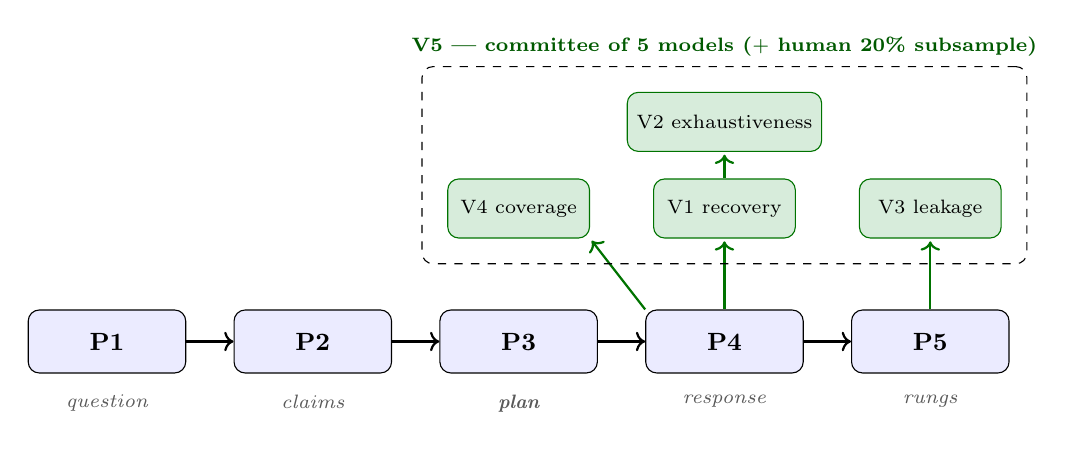
\begin{tikzpicture}[
  node distance=6mm,
  gen/.style={draw,rounded corners,minimum height=8mm,minimum width=20mm,
              font=\small\bfseries,fill=blue!8},
  val/.style={draw,rounded corners,minimum height=7.5mm,minimum width=18mm,
              font=\scriptsize,fill=cNew,draw=green!45!black},
  art/.style={font=\scriptsize\itshape,text=black!65},
  gate/.style={->,green!45!black,thick,shorten >=1pt},
  flow/.style={->,thick},
]
% generation chain
\node[gen] (p1) {P1};
\node[gen,right=of p1] (p2) {P2};
\node[gen,right=of p2] (p3) {P3};
\node[gen,right=of p3] (p4) {P4};
\node[gen,right=of p4] (p5) {P5};
\draw[flow] (p1) -- (p2);
\draw[flow] (p2) -- (p3);
\draw[flow] (p3) -- (p4);
\draw[flow] (p4) -- (p5);
% artefact labels underneath
\node[art,below=1.5mm of p1] {question};
\node[art,below=1.5mm of p2] {claims};
\node[art,below=1.5mm of p3] {\textbf{plan}};
\node[art,below=1.5mm of p4] {response};
\node[art,below=1.5mm of p5] {rungs};
% validators above, attached where they gate
\node[val,above=9mm of p3] (v4) {V4 coverage};
\node[val,above=9mm of p4] (v1) {V1 recovery};
\node[val,above=20mm of p4] (v2) {V2 exhaustiveness};
\node[val,above=9mm of p5] (v3) {V3 leakage};
\draw[gate] (p4.north) -- (v1.south);
\draw[gate] (v1.north) -- (v2.south);
\draw[gate] (p4.north west) -- (v4.south east);
\draw[gate] (p5.north) -- (v3.south);
% V5 as the committee running all validators
\node[draw,dashed,rounded corners,fit=(v4)(v2)(v3),inner sep=3.2mm,
      label={[font=\scriptsize\bfseries,text=green!35!black]above:%
      V5 --- committee of 5 models ($+$ human 20\% subsample)}] {};
\end{tikzpicture}
\caption{The generation pipeline (blue, left to right) and the admission gates (green, above).
\textsc{p1}--\textsc{p5} produce data; \textsc{v1}--\textsc{v4} decide whether an item is
admitted, and \textsc{v5} is the committee that runs them. \textsc{v1} is the load-bearing
gate: it re-derives the relation graph from the response \emph{without seeing the plan}, which
is what proves the gold is recoverable from the text rather than merely asserted about it.
\textsc{v2} runs on \textsc{v1}'s conflict edges only, adjudicating the exhaustiveness boundary
that separates \cCon\ from \cExc.}
\label{fig:pipeline}
\end{figure}

\begin{table}[h]\centering\small
\renewcommand{\arraystretch}{1.15}
\begin{tabular}{@{}llp{3.05cm}p{3.05cm}p{3.4cm}@{}}
\toprule
\textbf{ID} & \textbf{Role} & \textbf{Inputs} & \textbf{Output} & \textbf{Gate}\\
\midrule
\multicolumn{5}{@{}l}{\emph{Generation --- these produce the data}}\\
\textsc{p1} & topic $\to$ question & \texttt{TOPIC} &
  one bracketed question & ---\\
\textsc{p2} & atomic claims & \texttt{QUESTION} &
  24 tagged claims $+$ 2 holdings & ---\\
\textbf{\textsc{p3}} & \textbf{relation plan} & \texttt{QUESTION}, \texttt{CLAIMS} &
  \textbf{JSON graph}: atoms, relations, non-relations &
  schema-valid; $\geq1$ each of Alternative, Disjunction, Restatement, Concession,
  Precedence/Succession\\
\textsc{p4} & response & \texttt{QUESTION}, \texttt{PLAN} &
  prose response, $\geq500$ words & \textsc{v1}, \textsc{v3}, \textsc{v4}\\
\textsc{p5} & perturbation & \texttt{RESPONSE}, \texttt{PLAN}, \texttt{OPERATOR} &
  perturbed response $+$ JSON diff &
  one operator applied; length within 15\%\\
\midrule
\multicolumn{5}{@{}l}{\emph{Validation --- these decide what is admitted}}\\
\textsc{v1} & relation recovery & \texttt{RESPONSE}, \texttt{ATOMS} &
  recovered relation list &
  \textbf{$\geq$80\% coupling, $\geq$70\% sense}, else drop the edge or regenerate\\
\textsc{v2} & exhaustiveness & \texttt{CLAIM\_A}, \texttt{CLAIM\_B}, \texttt{RESPONSE} &
  one of A/B/C/D &
  \textbf{unanimity} for an \cExc\ label (Section~\ref{sec:risks}, R1)\\
\textsc{v3} & naturalness, leakage & \texttt{RESPONSE} &
  3 scores $+$ 3 span lists &
  all scores $\geq4$; leakage and hedging empty\\
\textsc{v4} & atom coverage & \texttt{RESPONSE}, \texttt{ATOMS} &
  per-atom status $+$ position &
  100\% \texttt{asserted}; positions re-verify the window\\
\midrule
\textsc{v5} & annotation protocol & --- & --- &
  \emph{not a prompt}: the committee and agreement thresholds
  (Section~\ref{sec:agreement})\\
\bottomrule
\end{tabular}
\caption{\textbf{The prompt suite index.} Full texts in Appendix~\ref{app:prompts}. Every
\texttt{NAME} above is a \texttt{[NAME\_PLACEHOLDER]} in the prompt body. Note \textsc{v5}
carries no prompt --- it is the protocol that runs \textsc{v1}--\textsc{v4}, kept in this series
because it is what makes their verdicts binding.}
\label{tab:promptindex}
\end{table}

% Float barrier: keep this section's tables inside it.
\clearpage

\subsection{Why P3 replaces LoReFact's logical-statement stage}
\label{sec:p3rationale}

The architectural departure is \textsc{p3}. \textsc{LoReFact} generates prose ``logical
statements'' and annotates them afterwards; we generate a \emph{machine-readable relation
graph} first and realize it in prose second. So the gold labels are an \textbf{input} to
generation rather than an output of annotation, which removes a whole class of annotation
error --- at the cost of requiring \textsc{v1} to prove the graph is actually recoverable from
the text.

That trade is worth making here for a reason specific to our taxonomy. Six of our thirteen
senses have no gold data anywhere (Table~\ref{tab:facetrel}), so post-hoc annotation would be
asking annotators to find relation facets they have never seen labelled, at whatever rate those
facets happen to occur in generated prose. Planning the graph first makes coverage of the
rare facets a \emph{generation constraint} (\textsc{p3} instruction 5) rather than a matter
of luck.

It also changes what \textsc{LoReFact}'s 78\%-false skew is for. Their skew follows from
instructing the generator that every logical statement must contain an error; ours is a
\texttt{validity} field with an explicit 55/45 target (\textsc{p3} instruction 8), so the
balance is a dial rather than a consequence.

\subsection{V5 --- the annotation protocol}
\label{sec:agreement}

\textsc{LoReFact} used three graduate-student annotators with a third-annotator tiebreak
(reaching 92.18\% agreement) plus a five-model committee with unweighted majority voting for
logical factuality. Ours mirrors that shape with two additions forced by our design.

\paragraph{Model committee (all items).} Five models drawn from at least three distinct
families, each running V1, V2 and V4 independently at temperature 0; per-edge label by
majority, ties escalated to a human. \textbf{Generation/validation disjointness:} the model
that ran P3/P4 for an item is \emph{excluded} from that item's committee, per R3.

\paragraph{Human annotation (stratified 20\%).} Three annotators on 120 items, stratified to
cover \emph{all} \cExc\ and \cCoN\ gold edges, all resolved Concessions, all \textsc{p-oo}
invariance rungs, and a random remainder. These are exactly the facets with no prior art
and the highest expected model unreliability, so uniform sampling would waste the human budget.

\paragraph{Statistics and thresholds.} Fleiss' $\kappa$ on the 13-way sense and 6-way coupling
labels (human-only and committee-only); Cohen's $\kappa$ on the binary exhaustiveness decision,
reported \emph{separately} as the expected weak point; Krippendorff's $\alpha$ (ordinal) on
strength bands; and human-versus-committee agreement, which is what licenses the committee as a
human proxy on the other 80\%. Acceptance: $\kappa \geq 0.70$ on coupling, $\geq 0.60$ on
sense, $\geq 0.55$ on exhaustiveness. A facet below threshold ships marked
\texttt{low\_agreement} and is excluded from headline metrics but reported as a finding --- an
unreliable facet is itself a result about the taxonomy.

% =====================================================================================
\section{The gold schema}
\label{sec:schema}

\subsection{A benchmark item}

The item format is a \textbf{strict superset} of \texttt{data/lcs/*.json}, so the nine shipped
fixtures remain valid and \texttt{RelationMiner.mine\_from\_atoms} loads a benchmark item
unchanged. Existing keys (\texttt{id}, \texttt{name}, \texttt{source}, \texttt{response},
\texttt{num\_atoms}, \texttt{atoms}, \texttt{notes}) keep their meaning; four blocks are added.

\begin{small}
\begin{verbatim}
{
  "id": "locobench-f012-r1",
  "name": "Aviation component failure - base",
  "source": "generated:P4/<model>@<date>",
  "response": "<full response text>",
  "num_atoms": 16,
  "atoms": [
    {"id": "a0", "text": "AeroParts supplied turbine blades to the carrier.",
     "label": "a1", "factual": true, "role": "claim",
     "sentence_index": 1, "char_span": [0, 52]}
  ],
  "notes": "...",

  "relations": [
    {
      "id": "r003",
      "source_id": "a10", "target_id": "a11",
      "level2_sense": "Alternative",
      "level1_coupling": "exclusive",
      "directed": false,
      "exhaustive": true,
      "ordering_only": false,
      "intended_strength_band": "strong",
      "strength_range": [0.85, 1.00],
      "validity": "valid",
      "error_kind": null,
      "is_concession": false,
      "is_resolved_concession": false,
      "resolver_atom_id": null,
      "position_distance": 1,
      "in_candidate_window": true,
      "window_admission": "window",
      "provenance": {
        "planned_by": "P3/<model>",
        "recovered_by": ["<m1>", "<m2>", "<m3>"],
        "recovery_rate": 0.80,
        "exhaustiveness_verdict": "A",
        "exhaustiveness_votes": {"A": 4, "B": 1, "C": 0, "D": 0},
        "human_confirmed": true,
        "annotator_agreement": 1.0,
        "low_agreement": false
      }
    }
  ],

  "non_relations": [
    {"source_id": "a1", "target_id": "a12", "position_distance": 3,
     "in_candidate_window": true,
     "provenance": {"recovered_as_none_by": 5, "human_confirmed": true}}
  ],

  "expected": {
    "family_id": "f012",
    "family_type": "F-CONF",
    "rung_index": 1,
    "rung_name": "base",
    "perturbation": {"operator": null, "target": null, "parent_rung": null},
    "readout_directions": {
      "mean_marginal": null, "consistency": null, "log_partition": null
    },
    "invariants": [],
    "reference_values": {
      "mean_marginal": 0.607, "consistency": null, "log_partition": -9.64
    }
  },

  "meta": {
    "domain": "Engineering & Technology",
    "topic": "aviation component failure investigation",
    "split": "test",
    "word_count": 623,
    "validation": {
      "v1_coupling_recall": 0.88, "v1_sense_recall": 0.75,
      "v3_fluency": 5, "v3_leakage": [], "v4_coverage": 1.0
    }
  }
}
\end{verbatim}
\end{small}

Field notes, in decreasing order of consequence:

\begin{description}[leftmargin=*,nosep]
  \item[\texttt{level1\_coupling}] must satisfy
        \texttt{COMPILE[level2\_sense].level1 == level1\_coupling}. A builder assertion
        \textbf{must} enforce this, so gold can never silently contradict
        \texttt{taxonomy.py} (Table~\ref{tab:compile}). The same applies to \texttt{directed}
        and \texttt{ordering\_only}, which mirror \texttt{SenseSpec}.
  \item[\texttt{exhaustive}] is meaningful only for \cCon/\cExc\ edges, where
        \texttt{true} $\Leftrightarrow$ Alternative. It is stored \emph{explicitly} rather than
        derived from the sense: that redundancy is deliberate, because it is what lets a
        disputed edge be flagged \texttt{low\_agreement} while still carrying a sense, and it
        is the field the exhaustiveness metric grades against.
  \item[\texttt{in\_candidate\_window} / \texttt{window\_admission}] (\texttt{window} $|$
        \texttt{gate} $|$ \texttt{discourse\_promoted} $|$ \texttt{out\_of\_window}) are
        computed at build time by actually running
        \texttt{candidate\_pairs.select(policy="gated", window=4)} and recording the verdict.
        This makes gold recoverability under the shipped pair policy an explicit, queryable
        property rather than an assumption (R2).
  \item[\texttt{readout\_directions}] carries the per-readout expectation from
        Table~\ref{tab:ops} for the perturbation that produced this rung --- one of
        \texttt{decrease}, \texttt{increase}, \texttt{invariant}, \texttt{unconstrained} per
        readout, relative to \texttt{parent\_rung}. It is \texttt{null} on a base rung. This is
        where Finding~1 lives in the data.
  \item[\texttt{role}] on an atom is \texttt{claim} $|$ \texttt{holding} $|$
        \texttt{distractor}, so a resolver can be located without re-running the heuristic.
\end{description}

\subsection{The family manifest}

\begin{small}
\begin{verbatim}
{
  "manifest_version": "1.0",
  "families": [
    {
      "family_id": "f012",
      "family_type": "F-CONF",
      "domain": "Engineering & Technology",
      "topic": "aviation component failure investigation",
      "rungs": [
        {"index": 0, "name": "worse",  "item_id": "locobench-f012-r0",
         "operator": "spurious_relation", "parent": 1},
        {"index": 1, "name": "base",   "item_id": "locobench-f012-r1",
         "operator": null, "parent": null},
        {"index": 2, "name": "concession_resolved", "item_id": "...-r2",
         "operator": "add_resolution", "parent": 1},
        {"index": 3, "name": "fix_one_conflict",    "item_id": "...-r3",
         "operator": "drop_relation",  "parent": 2},
        {"index": 4, "name": "coherent",            "item_id": "...-r4",
         "operator": "drop_relation",  "parent": 3}
      ],
      "ordering_constraints": [
        {"id": "c1", "class": "C1",
         "readouts": ["mean_marginal", "log_partition"],
         "chain": [0, 1, 2, 3, 4], "strict": true},
        {"id": "c2", "class": "C2",
         "readouts": ["consistency"],
         "required": [[0, 1], [3, 4]],
         "expected_inversions": [[1, 2]],
         "unconstrained": [[2, 3]]},
        {"id": "c3", "class": "C3",
         "readouts": ["mean_marginal", "consistency", "log_partition"],
         "required": [[0, 4]], "strict": true}
      ],
      "invariance_constraints": [],
      "noise_sigma": {"mean_marginal": 0.004, "consistency": 0.011,
                      "log_partition": 0.06},
      "margin_rule": "abs_delta > 2 * noise_sigma else indeterminate"
    }
  ],
  "legacy_pairs": [
    {"family_id": "seed-renda",
     "rungs": [{"index": 0, "item_id": "example-5-renda-S"},
               {"index": 1, "item_id": "example-5-renda-K"}],
     "ordering_constraints": [{"id": "c3", "class": "C3",
       "readouts": ["mean_marginal"], "required": [[0, 1]], "strict": true}]},
    {"family_id": "seed-biography",
     "rungs": [{"index": 0, "item_id": "example-2-biography-contradicted"},
               {"index": 1, "item_id": "example-2-biography"}],
     "ordering_constraints": [{"id": "c3", "class": "C3",
       "readouts": ["mean_marginal"], "required": [[0, 1]], "strict": true}]}
  ]
}
\end{verbatim}
\end{small}

\texttt{expected\_inversions} in the \texttt{c2} constraint is Finding~1 made executable: the
harness \emph{asserts} that \readout{consistency} falls from rung 1 to rung 2, rather than
exempting the step.

\subsection{Migrating the seed fixtures}
\label{sec:migration}

\texttt{scripts/build\_lcs\_examples.py} already contains hand-authored gold relations, as
4-tuples \texttt{(src\_label, trg\_label, level1\_type, relation\_class)} with
\texttt{relation\_class} $\in$ \{\texttt{prerequisite}, \texttt{invalidation}\} --- and
\texttt{\_build\_record} \textbf{discards them}. The comment at its definition promises they
are ``expanded to a0-based ids at build time''; that expansion was never implemented, so the
data is live only inside the script. Phase 1 specifies surfacing it:

\begin{itemize}[leftmargin=*,nosep]
  \item \texttt{prerequisite} $\rightarrow$ \texttt{level2\_sense: "Cause-Effect"},
        \texttt{level1\_coupling: "entailment"}, \texttt{directed: true};
  \item \texttt{invalidation} $\rightarrow$ \texttt{"Contrast"}, \cCon, \texttt{directed: false};
  \item the AeroParts \texttt{equivalence} edge $\rightarrow$ \texttt{"Restatement"}, \cEqv;
  \item the AeroParts blame conflict additionally gets \texttt{is\_concession: true},
        \texttt{is\_resolved\_concession: true} and its \texttt{resolver\_atom\_id}, per the
        fixture's existing \texttt{notes}.
\end{itemize}

\paragraph{Why this makes the seed set dev, not test.} The migration is \textbf{lossy in sense
granularity}: \texttt{prerequisite} covers whatever the true sense was, so mapping it to
Cause-Effect is a guess wherever the truth is Evidence, Condition or Instantiation. Migrated
edges are therefore graded on \textbf{coupling only} unless a human re-annotates the sense.
Migrated edges carry \texttt{provenance.planned\_by: "hand-authored"} and must still pass V1 to
be scored.

\paragraph{Two housekeeping items to resolve before Phase 2 touches that script.}
\texttt{data/lcs/example-6-incident.json} is \textbf{orphaned}: the builder registers only
eight examples and does not know it, and \texttt{data/lcs/README.md} omits it. Separately, that
README has been \textbf{hand-edited since generation} --- it documents the two-stage
\texttt{node\_priors} path that \texttt{\_write\_readme} does not emit --- so re-running the
builder would regress it. Either fold example 6 into the builder and re-sync the README
generator, or move both under the new benchmark builder.

% =====================================================================================
\section{Metrics}
\label{sec:metrics}

Notation: item $k$ has gold edge set $G_k$ and candidate-pair set $C_k$; a system produces
predicted edges $P_k$. Let $G^{\text{edge}}$ be the gold edges with a non-\cNone\ coupling, and
$N$ the \texttt{non\_relations} pool. Write $c, s, d$ for gold coupling/sense/direction and
$\hat c, \hat s, \hat d$ for predictions.

\paragraph{All Target-A metrics are computed over candidate pairs only.} A pair the policy never
scored cannot be a miner error. Gold edges with
\texttt{in\_candidate\_window: false} are excluded from recall and reported separately as the
\textbf{structural-miss rate} --- conflating the two would blame the miner for the gate's
decisions (R2).

\subsection{Target A --- the miner as a classifier}
\label{sec:metrics-a}

\begin{enumerate}[leftmargin=*,nosep,label=\textbf{A\arabic*.}]
  \item \textbf{Coupling accuracy.}
        $\mathrm{CouplingAcc} = |\{e \in G^{\text{edge}} : \hat c(e) = c(e)\}| \,/\, |G^{\text{edge}}|$.
  \item \textbf{Sense accuracy.} Same denominator with $\hat s, s$. Report also
        \textbf{SenseAcc-hard}, restricted to edges whose confusability weight is 3
        (Table~\ref{tab:confuse}), and split every figure into
        \emph{coupling-changing} versus \emph{coupling-preserving} confusions.
  \item \textbf{Direction accuracy.} Over gold edges where
        \texttt{COMPILE[s].directed} holds \emph{and} the coupling was predicted correctly
        (direction on a wrong coupling is not meaningful):
        \[
          \mathrm{DirAcc} = \frac{|\{e : \hat d(e) = d(e) \wedge \hat c(e) = c(e)\}|}
                                 {|\{e \in G : \texttt{directed}(s(e))\}|}.
        \]
  \item \textbf{None-detection P/R/F1.} With $P_{\text{none}}$ the pairs the system labels
        \cNone:
        \[
          \mathcal{P} = \frac{|N \cap P_{\text{none}}|}{|P_{\text{none}}|}, \qquad
          \mathcal{R} = \frac{|N \cap P_{\text{none}}|}{|N|}, \qquad
          F_1 = \frac{2\mathcal{P}\mathcal{R}}{\mathcal{P}+\mathcal{R}}.
        \]
        Note $1 - \mathcal{P}$ \textbf{is} the over-connection rate --- our documented failure
        mode, and the reason the \texttt{None} pool is first-class data
        (Section~\ref{sec:counts}).
  \item \textbf{Exhaustiveness accuracy.} Over gold edges with coupling $\in$ \{\cCon, \cExc\},
        the rate at which \texttt{exhaustive} is predicted correctly, \emph{plus} the explicit
        $2\times2$ Contrast/Alternative confusion matrix. This metric has no \textsc{LoReFact}
        analogue and is the one that justifies \cExc\ as a separate coupling.
  \item \textbf{Concession-resolution accuracy.} Over gold \texttt{is\_concession} edges: the
        binary ``did the system mark it resolved'', reported separately from exact
        \texttt{resolver\_atom\_id} match.
  \item \textbf{Strength-band agreement.} Exact-match rate; \emph{adjacent} accuracy
        (off-by-one band counted correct); Krippendorff's $\alpha$ (ordinal); and the mean
        absolute deviation of the predicted $p$ from the nearest edge of the gold band, zero
        inside the band.
  \item \textbf{Confusion matrices.} $13\times13$ over senses and $6\times6$ over couplings,
        each with an extra \texttt{structural} row/column for out-of-window gold. Published as
        the primary diagnostic artifact --- the aggregate numbers above are summaries of it.
\end{enumerate}

\subsection{LoReFact-comparable analogues}
\label{sec:analogues}

\textsc{LoReFact}'s three headline logic metrics, lifted to a graded, graph-level setting
(Table~\ref{tab:analogue}). The point of this table is comparability: a reader of both papers
should be able to line the numbers up.

\begin{table}[h]\centering\small
\renewcommand{\arraystretch}{1.15}
\begin{tabular}{@{}llp{7.6cm}@{}}
\toprule
\textbf{\textsc{LoReFact}} & \textbf{LoCoBench} & \textbf{Definition and difference}\\
\midrule
LogicRecall & \textbf{EdgeRecall} &
  $|\{e \in G^{\text{edge}} : \hat c(e) \neq \cNone\}| / |G^{\text{edge}}|$ --- fraction of
  in-window gold edges detected as \emph{some} relation. Complements $\mathcal{R}$ above\\
LogicTypeAcc & \textbf{CouplingAcc}, \textbf{SenseAcc} &
  their 5-class becomes our 6-class coupling and 13-class sense, i.e.\ two granularities
  instead of one\\
LogicFactualityAcc & \textbf{ValidityAUROC}, \textbf{BandMAE} &
  their binary ``does the dependency hold'' becomes graded: use the miner's edge probability
  $p$ as a score for \texttt{validity} and report AUROC. A thresholded
  \textbf{ValidityAcc} at $p{=}0.5$ is also reported for direct numeric comparison\\
\midrule
--- & \textbf{CoherenceAUC} &
  new: pooling all items, each readout used as a score for ``this rung is in the top half of
  its family''. One number per readout, comparable across readouts \emph{and} against
  DiscoScore / G-Eval / SelfCheckGPT-NLI\\
\bottomrule
\end{tabular}
\caption{\textsc{LoReFact} metric analogues. The graded-versus-binary shift in the third row is
the substantive one: a binary logic-factuality label discards exactly the information our
relation probability carries.}
\label{tab:analogue}
\end{table}

\subsection{Target B --- readout ranking}
\label{sec:metrics-b}

For readout $\rho$ and family $f$ with rungs $r_0..r_4$, and $\sigma_\rho$ the measured
run-to-run noise:

\begin{enumerate}[leftmargin=*,nosep,label=\textbf{B\arabic*.}]
  \item \textbf{Pairwise ranking accuracy}, over the constraint's required pairs, excluding
        indeterminate ones:
        \[
          \mathrm{PRA}(\rho) =
          \frac{\sum_f |\{(i,j) \text{ required} : \rho(r_j) - \rho(r_i) > 2\sigma_\rho\}|}
               {\sum_f |\{(i,j) \text{ required} : \text{determinate}\}|}.
        \]
        \textbf{Must be reported with the indeterminate rate.} A system can score
        $\mathrm{PRA}=1$ trivially by being noisy enough that every pair is indeterminate; the
        two numbers are only meaningful together.
  \item \textbf{Kendall $\tau$-b} between the readout's rung ordering and the gold rung index,
        per family, averaged. Computed on the full C1 chain for \readout{mean\_marginal} and
        \readout{log\_partition}; on the C2-required sub-chain only for \readout{consistency}
        since $\tau$ over the full chain is not meaningful given the
        predicted inversion.
  \item \textbf{Monotonicity violation rate.} Fraction of C1 adjacent pairs moving the wrong
        way by more than $2\sigma_\rho$. Strict violations only --- noise-level wobble is not a
        violation.
  \item \textbf{Quirk-conformity rate} (C2, \readout{consistency} only).
        Fraction of families where the readout \emph{does} invert at rung $1\to2$ as
        Finding~1 predicts. \textbf{Target is high, not low}: a system monotone here is not
        implementing the concession discount.
  \item \textbf{Invariance pass rate.} Over \textsc{p-oo} and \textsc{p-dr} rungs,
        $\mathrm{INV}(\rho) = |\{\,|\rho(\text{perturbed}) - \rho(\text{parent})| \leq
        2\sigma_\rho\}| / |\text{items}|$, reported separately as \textsc{inv-ordering} and
        \textsc{inv-direction}. This is the one metric where all three readouts share the same
        strict expectation; a \textsc{inv-direction} failure means the factor tables have become
        direction-sensitive.
  \item \textbf{Endpoint separation and dynamic range.} $\rho(r_4) - \rho(r_0)$, mean and
        distribution, plus the 5th/95th percentile of $\rho$ over all items. The reference
        family spans only $0.586$--$0.620$, so a \emph{compressed} range is expected and must be
        quantified rather than treated as a defect.
  \item \textbf{Human correlation.} Spearman $\rho$ between each readout and human coherence
        ratings on the 120-item human subsample, against DiscoScore \citep{discoscore}, the
        G-Eval coherence dimension \citep{geval} and SelfCheckGPT-NLI \citep{selfcheckgpt}, per
        \texttt{research\_plan.md}~\S9.
\end{enumerate}

\begin{table}[h]\centering\small
\renewcommand{\arraystretch}{1.1}
\begin{tabular}{@{}lccc@{}}
\toprule
\textbf{Metric} & \readout{mean\_marginal} & \readout{consistency} &
\readout{log\_partition}\\
\midrule
PRA, C1 chain                & \checkmark & --- & \checkmark\\
PRA, C2 required             & \checkmark & \checkmark & \checkmark\\
Kendall $\tau$               & full & sub-chain & full\\
Monotonicity violation       & \checkmark & --- & \checkmark\\
Quirk conformity             & --- & \checkmark & ---\\
Invariance (\textsc{p-oo}, \textsc{p-dr}) & \checkmark & \checkmark & \checkmark\\
Endpoint separation (C3)     & \checkmark & \checkmark & \checkmark\\
Human Spearman               & \checkmark & \checkmark & \checkmark\\
\bottomrule
\end{tabular}
\caption{Metric applicability by readout, following from the C1/C2/C3 contract classes of
Section~\ref{sec:contracts}. Target-A metrics are deliberately absent: they grade the miner
upstream of scoring, so a miner regression is diagnosable without re-running inference.}
\label{tab:applic}
\end{table}

% =====================================================================================
% Float barrier: keep this section's tables inside it.
\clearpage

\section{Risks and Phase-2 open questions}
\label{sec:risks}

\paragraph{R1 --- LLM-generated exhaustiveness may be unreliable (highest risk).}
Deciding Contrast versus Alternative requires quantifying over possible worlds, which models
handle poorly, and it is exactly the boundary where \cExc\ earns its existence as a separate
coupling. Mitigations: V2's explicit ``coherent third state'' procedure; \textbf{unanimity}
(not majority) of the committee required for an \cExc\ gold label; 100\% human coverage of
those edges in the subsample; \texttt{low\_agreement} flagging. \emph{Fallback:} seed
Alternative edges from \textbf{structurally guaranteed} pairs --- numeric or polarity
complements (``no one was harmed'' / ``three people died''), where exhaustiveness follows from
the semantics of negation rather than from world knowledge. \emph{Open:} if human $\kappa$ on
exhaustiveness lands below $0.55$, is \cExc\ a defensible benchmark facet at all, or should
it ship as a research-only subset?

\paragraph{R2 --- the candidate window versus gold recoverability.}
Under \texttt{policy="gated", window=4}, a gold edge whose endpoints are more than 4 positions
apart and which fails both the similarity gate and the discourse-adjacency check is
\textbf{unmineable by construction}. Handled in three places: P3 instruction 4 biases generation
into the admissible set; build time records \texttt{in\_candidate\_window} /
\texttt{window\_admission} per edge by running the real selector; the metrics exclude
out-of-window gold and report the structural-miss rate separately. \emph{Open:} P3 constrains
\emph{planned} positions but P4's realized order may drift, so V4's \texttt{position} output must
re-verify the constraint post hoc and items that break it must regenerate. \emph{Also open:}
should Phase 2 ship a deliberate \texttt{long\_range} subset of out-of-window gold to grade
\emph{the gate itself} as a retrieval problem (precision/recall of admission)? That is a
different and probably valuable evaluation, and the schema already supports it.

\paragraph{R3 --- self-generation bias.}
If the same model family generates (P3/P4) and mines (Prompt A/B), the miner may recover its own
lexical fingerprints rather than genuine discourse structure, inflating every Target-A number.
Mitigations: per-item generator exclusion from the validation committee
(Section~\ref{sec:agreement}); the generator recorded in \texttt{source} and stratified across
$\geq 3$ families so per-generator breakdowns are computable; and a \textbf{cross-generation
control} --- Target-A reported both pooled and restricted to items whose generator family
differs from the miner's, with the gap published as a bias estimate. \emph{Open (recommended
yes):} a small human-authored slice, say 50 items with no LLM generation at any stage, as an
unbiased anchor. It is cheap relative to its diagnostic value, and the nine existing fixtures
are a precedent for the format.

\paragraph{R4 --- Restatement's strength prior.}
Per Finding~2 (Section~\ref{sec:finding-prior}) the $0.90$ prior is unreachable on the
production path, so it cannot be tested through the pipeline. What Phase 2 \emph{can} report is
the distribution of mined strength on gold Restatement edges --- i.e.\ whether $0.90$ is
empirically justified. \emph{Open:} if mined Restatement strength centres well away from
$0.90$, the prior should be re-estimated or removed rather than left as unreachable code.

\paragraph{R5 --- the MLN formulation cannot be benchmarked end to end.}
\texttt{formulation="mln"} constructs but raises at \texttt{score()}, and \cExc\ / \cCoN\ raise
in that path specifically. Target B is therefore scoped to the MRF. The MLN's closed-form
pairwise fragment is verified to reproduce the MRF exactly, so nothing is lost for the pairwise
facets; beyond-pairwise structure is out of scope until an engine exists.

\paragraph{R6 --- generation cost.}
\textsc{LoReFact} reports $\approx$110 LLM calls and $\approx$\$0.32 per sample for their
\emph{evaluation} pipeline alone. Ours adds a 5-model validation committee over V1/V2/V4 and a
5-rung ladder per family. Phase 2 should cost the run before committing to 600 items, and the
schema's \texttt{reference\_values} exist partly so that cheap dry-run scoring (the brute-force
oracle, and \texttt{score\_all}'s shared base inference) can substitute during harness
development.

On the inference side the three-readout scope (Section~\ref{sec:scope}) costs \textbf{5 Merlin
calls per item}, not 6: a base MAR and a base PR shared by all three, plus
\readout{consistency}'s U-chain MAR and \readout{log\_partition}'s contradiction-free ceiling PR
and saturated-floor MAP. Excluding \texttt{reified} removes exactly its R-node MAR run. Over 600
items $\times$ 5 rungs that is 3{,}000 items and $\approx$15{,}000 Merlin invocations, so the
saving is real but second-order next to the LLM committee cost above.

% =====================================================================================
\section{Summary of Phase-1 decisions}
\label{sec:summary}

\begin{enumerate}[leftmargin=*,nosep,label=\arabic*.]
  \item \textbf{Two gradable targets}, not one: per-pair relation labels (A) grade the miner as
        a classifier; coherence-ordered families (B) grade the three readouts by ranking. A
        alone would leave the score untested; B alone would give no diagnosis of \emph{which}
        facets fail.
  \item \textbf{Thirteen senses, five couplings}, exactly as \texttt{taxonomy.py} defines them,
        with \cEqv, \cExc\ and \cCoN\ over-represented because no prior gold data exists for
        them.
  \item \textbf{Two orthogonal organizations, named apart.} \emph{Facets} are LoCoBench's own
        structural axes (relation, item, annotation); \emph{topic} and \emph{domain} stay
        reserved for the 36 subjects inherited from \textsc{LoReFact}, \textbf{all of which must
        be represented}. Both are coverage requirements, and both are reported --- a
        topic breakdown says whether the benchmark generalizes across subject matter, a facet
        breakdown says which structural phenomena a scorer handles.
  \item \textbf{Validity-balanced, not false-skewed}: 55/45 valid/invalid with a coherent and a
        maximally-perturbed rung in every family, departing deliberately from
        \textsc{LoReFact}'s 78\% because a graded score must be validated at both ends.
  \item \textbf{A relation plan replaces prose logical statements}: gold is an \emph{input} to
        generation, gated by a round-trip recovery check rather than produced by post-hoc
        annotation.
  \item \textbf{Per-readout ordering contracts} (C1/C2/C3), because one of the three readouts
        provably invert at the concession rung and a global monotonicity requirement would fail
        a correct implementation.
  \item \textbf{Two strict invariance tests} --- ordering-only and direction-reversal --- which
        are the design's sharpest instruments because a prediction of \emph{no effect} cannot be
        satisfied by accident.
  \item \textbf{A superset schema}, so the nine shipped fixtures become the dev split with no
        format fork, graded on coupling only where their migration is lossy.
\end{enumerate}

Phase 2 is the generation run: topic selection, the live prompt pipeline, the validation
committee, and the harness that turns \texttt{expected} blocks into assertions.

% =====================================================================================
\begin{thebibliography}{9}\small

\bibitem[LoReFact]{lorefact} Q.~Xie, W.~Zheng, X.~Shen, and R.~Xia.
  \emph{LoReFact: Bridging the Logic Gap in Fact-Checking.}
  Findings of the Association for Computational Linguistics: ACL 2026, pages 6974--6996, 2026.

\bibitem[FactReasoner]{factreasoner} R.~Marinescu et al.
  \emph{FactReasoner: A Probabilistic Approach to Long-Form Factuality Assessment for Large
  Language Models.} arXiv:2502.18573, 2025.

\bibitem[DiscoScore]{discoscore} W.~Zhao, M.~Strube, and S.~Eger.
  \emph{DiscoScore: Evaluating Text Generation with BERT and Discourse Coherence.}
  arXiv:2201.11176, 2023.

\bibitem[G-Eval]{geval} Y.~Liu, D.~Iter, Y.~Xu, S.~Wang, R.~Xu, and C.~Zhu.
  \emph{G-Eval: NLG Evaluation using GPT-4 with Better Human Alignment.}
  arXiv:2303.16634, 2023.

\bibitem[SelfCheckGPT]{selfcheckgpt} P.~Manakul, A.~Liusie, and M.~J.~F.~Gales.
  \emph{SelfCheckGPT: Zero-Resource Black-Box Hallucination Detection for Generative Large
  Language Models.} arXiv:2303.08896, 2023.

\bibitem[PDTB3]{pdtb} R.~Prasad, B.~Webber, and A.~Lee.
  \emph{Penn Discourse Treebank Version 3.0.} LDC2019T05, Linguistic Data Consortium, 2019.

\bibitem[Barzilay]{barzilay} R.~Barzilay and M.~Lapata.
  \emph{Modeling Local Coherence: An Entity-Based Approach.}
  Computational Linguistics, 34(1):1--34, 2008.

\bibitem[Li]{li} J.~Li and D.~Jurafsky.
  \emph{Neural Net Models of Open-Domain Discourse Coherence.}
  EMNLP 2017.

\bibitem[SAFE]{safe} J.~Wei et al.
  \emph{Long-Form Factuality in Large Language Models.} NeurIPS 2024.

\end{thebibliography}

% =====================================================================================
\appendix
\section{The prompts, verbatim}
\label{app:prompts}

The nine prompts of Table~\ref{tab:promptindex}, copy-ready. Each is preceded by its contract:
the placeholders it takes, the output it must produce, and the gate its output must pass.
Generation prompts (\textsc{p1}--\textsc{p5}) come first, then validation
(\textsc{v1}--\textsc{v4}). \textsc{v5} is not a prompt and is specified in
Section~\ref{sec:agreement}.

\subsection{P1 --- topic to question}

\promptsig{P1 --- topic to question}{\texttt{[TOPIC\_PLACEHOLDER]} --- one of the 36 subject
topics of Table~\ref{tab:topics}. The prompt is run per topic, so \emph{topic selection is not
the prompt's job}: instruction 4's preference for adjudicated framings applies \emph{within}
whatever topic it is given, and never substitutes for covering all
36 (Section~\ref{sec:subjects}).}{One question, wrapped in square brackets, no
preamble.}{None. A weak question is caught downstream by \textsc{p3} failing instruction 5.}

\begin{small}
\begin{verbatim}
Instructions:
1. You are given a TOPIC. Generate one open-ended QUESTION about that topic.
2. The QUESTION must begin with Why, How, What, Does, or Which.
3. The QUESTION must elicit an answer containing MULTIPLE, DIVERSE logical
   relationships. Aim for an answer that would naturally contain at least four
   of the following: a causal chain; a condition; a temporal ordering; an
   evidential appeal; a general claim with a specific instance; a restatement
   or definitional equivalence; a non-exhaustive contrast; an EXHAUSTIVE pair
   of competing alternatives of which EXACTLY ONE can hold; a disjunctive pair
   of which AT LEAST ONE must hold; a tension that an authoritative finding
   later resolves.
4. Prefer topics where competing explanations are adjudicated: incident
   investigations, litigation, diagnostic reasoning, attribution disputes,
   competing scientific hypotheses. Such topics naturally produce exhaustive
   alternatives and resolving holdings.
5. The QUESTION must be answerable in 500-900 words of formal prose.
6. The QUESTION must not itself contain the words "cause", "condition",
   "alternative", or "contrast", so the answer's relations are not primed
   lexically.
7. Do NOT ask a multi-part question joined by "and" - one question only.
8. Wrap the QUESTION in square brackets.
9. Output the bracketed QUESTION only, with no preamble.

Use the following examples to better understand your task.

TOPIC: aviation component failure investigation
QUESTION: [How do investigators determine responsibility when a component
supplied by a third party fails in service and the operator and the
manufacturer offer competing explanations?]

TOPIC: antibiotic resistance in hospital settings
QUESTION: [Why does resistance emerge in some hospital units but not others,
and how is a specific outbreak traced to its origin?]

Your Task:
TOPIC: [TOPIC_PLACEHOLDER]
QUESTION:
\end{verbatim}
\end{small}

Instructions 3 and 4 are the substantive extension of \textsc{LoReFact}'s Table 11, which asks
only for ``causal, conditional, or temporal reasoning''. Instruction 4 encodes an empirical
bet: adjudicated domains are where exhaustive alternatives and resolving holdings occur
naturally, so steering topic selection is cheaper than forcing the structure later.
Instruction 6 prevents lexical priming that would make the miner's job artificially easy.

\subsection{P2 --- atomic claim generation}

\promptsig{P2 --- atomic claim generation}{\texttt{[QUESTION\_PLACEHOLDER]}.}{A markdown code block: 24 claims as \texttt{-} bullets, each with one of the 9 tags of Table~\ref{tab:facetann}, plus 2 \texttt{[holding]} claims.}{Composition must match instruction 3 exactly (14 correct, 4 incorrect, and the alt/disj/equiv pairs); the holdings must use adjudicating vocabulary.}

\begin{small}
\begin{verbatim}
Instructions:
1. You are given a QUESTION. Generate a set of ATOMIC CLAIMS that a
   well-informed answer to it might contain.
2. An atomic claim is a sentence containing a singular piece of information,
   which should be basic, indivisible, and independently verifiable.
3. Generate exactly 26 atomic claims: the 24 below, plus the 2 holding claims
   required by instruction 4. The 24 break down as:
   (a) 14 factually correct claims;
   (b) 4 factually incorrect claims (plausible but false);
   (c) 2 EXHAUSTIVE ALTERNATIVE claims: a pair X, Y such that exactly one of X
       and Y must be true - they cannot both hold, and they cannot both fail.
       Example pair: "No one was harmed in the incident." / "Three people died
       in the incident."
   (d) 2 DISJUNCTIVE claims: a pair X, Y such that at least one must be true,
       but both may be true simultaneously. Make each one a STATE OF THE WORLD,
       not a finding or a check that reported something: "the alloy was
       substituted" and "the batch was mislabelled", not "assay A flagged it"
       and "assay B flagged it".
   (e) 2 EQUIVALENT claims: a pair X, Y asserting the same fact in different
       words, so that either one being true makes the other true.
4. Additionally generate 2 HOLDING claims: sentences in which an authority
   (a court, tribunal, regulator, final report, or review board) reaches a
   determination that settles a dispute between two other claims in your list.
   A holding claim must use adjudicating language - "held", "ruled",
   "concluded", "determined", "found that", "ultimately".
5. Each claim must be a single declarative sentence with no connective linking
   it to another claim. Do NOT use "because", "although", "therefore", "if",
   "while", "however". Relations are added at a later stage, not here.
6. Do NOT indicate which claims are factually incorrect in their wording; do
   NOT hedge with "assume", "might", "possibly", or "allegedly".
7. Output as a markdown code block: an unordered list with "-" bullets. Append
   a tag in square brackets to every claim, one of: [correct], [incorrect],
   [alt-pair-1], [alt-pair-2], [disj-pair-1], [disj-pair-2], [equiv-pair-1],
   [equiv-pair-2], [holding].

Use the following example to better understand your task.

QUESTION: [How do investigators determine responsibility when a component
supplied by a third party fails in service and the operator and the
manufacturer offer competing explanations?]

ATOMIC CLAIMS:
```
- AeroParts supplied turbine blades to the carrier. [correct]
- The turbine blades were installed in the carrier's A-320 fleet. [correct]
- Seventeen turbine blades failed in flight during service. [correct]
- The regulator opened a safety probe into the blade failures. [correct]
- Maintenance logs recorded abnormal vibration on the failed blades. [correct]
- The airline argued that the failures were caused by pilot error. [correct]
- The final report concluded the root cause was a metallurgical defect. [correct]
- The regulator issued an order grounding the fleet. [correct]
- Every affected aircraft was pulled from service. [equiv-pair-1]
- The regulator's order removed all affected aircraft from operation. [equiv-pair-2]
- The blades were certified under a 1998 airworthiness standard. [incorrect]
- No one was harmed in the incidents. [alt-pair-1]
- Three passengers died in one of the failures. [alt-pair-2]
- The alloy supplied for the blades was substituted. [disj-pair-1]
- The blade batch was mislabelled at the mill. [disj-pair-2]
- The tribunal held that AeroParts was liable for the blade failures. [holding]
- The accident report found the pilots not at fault. [holding]
```

Your Task:
QUESTION: [QUESTION_PLACEHOLDER]
ATOMIC CLAIMS:
\end{verbatim}
\end{small}

Instruction 3(c)--(e) and instruction 4 are the extension. \textsc{LoReFact}'s Table 12 asks
for 10 correct and 10 incorrect claims and nothing else; its instruction that claims be
``independently verifiable'' actively \emph{precludes} the equivalent pairs an \cEqv\ edge
needs. The tagged pairs are the raw material for the three couplings with no prior gold, and
the \texttt{[holding]} claims are what make a \emph{resolved} Concession constructible. Their
required vocabulary is not stylistic: it matches the cue list in the miner's
\texttt{\_looks\_like\_holding} heuristic (\texttt{held}, \texttt{ruled}, \texttt{concluded},
\texttt{tribunal}, \texttt{determined}, \ldots), so a planned resolution is one the shipped
resolver can actually find. Instruction 5 is load-bearing in the other direction: claims must
arrive \emph{connective-free} so that every relation in the final response traces to P3's plan
rather than to an accident of claim phrasing.

\subsection{P3 --- relation plan generation}

\promptsig{P3 --- relation plan generation \textnormal{(the architectural departure, Section~\ref{sec:p3rationale})}}{\texttt{[QUESTION\_PLACEHOLDER]}, \texttt{[CLAIMS\_PLACEHOLDER]} (P2s tagged list).}{One JSON object: \texttt{atoms} (with \texttt{pos}), \texttt{relations} (sense, strength band, validity, error kind, resolver), \texttt{non\_relations}.}{Schema-valid; $\geq1$ each of Alternative, Disjunction, Restatement, Concession and Precedence/Succession (instr.~5); 6 valid / 4 invalid of 10 relations (instr.~8). Locality (instr.~4) is \emph{recorded, not enforced} here --- see R2.}

This replaces \textsc{LoReFact}'s logical-statement stage (their Table 13). Their stage emits
prose and requires that ``each logical statement must contain a logical error'', which is what
produces their 78\% skew. Ours emits a graph and controls the valid/invalid ratio explicitly.

\begin{small}
\begin{verbatim}
Instructions:
1. You are given a QUESTION and a tagged list of ATOMIC CLAIMS. Produce a
   RELATION PLAN: a machine-readable graph of the logical relations a response
   should draw between those claims.
2. Select 14-16 claims to use. Aim for 15. Number them with FRESH consecutive
   positions: the first claim you assert is pos 1, the next pos 2, and so on
   with NO gaps and NO repeats, ending at pos N where N is how many you
   selected. Do NOT carry over the numbering of the input list - if you pick the
   3rd, 7th and 12th claims they become pos 1, 2 and 3. The position is the
   order the response will assert the claim in. Every selected claim keeps its
   text EXACTLY as given. Do NOT introduce information not in the claims, and
   do NOT alter the claims. Your selection MUST INCLUDE AT LEAST 2 of the
   [incorrect] claims: the response has to assert false content alongside the
   true, so a selection drawn only from the [correct] claims is rejected. Carry
   each selected claim's tag through as a "factual" field - false for an
   [incorrect] claim, true for every other tag.
3. Plan EXACTLY 10 RELATIONS. Each relation connects exactly two selected claims
   and has a SENSE. Every relation must join a DIFFERENT pair of claims: once two
   claims are related, that pair is used up and must not appear again in the
   relations list, in either direction. The SENSE is one of: Cause-Effect,
   Effect-Cause, Evidence, Condition,
   Restatement, Instantiation, Contrast, Concession, Alternative, Disjunction,
   Precedence, Succession.
   - Cause-Effect: source causes target. Effect-Cause: source is the effect,
     target its cause.
   - Evidence: source is evidence for target. Condition: source is a condition
     for target.
   - Restatement: source and target assert the same thing.
   - Instantiation: source is a general claim, target a specific instance.
   - Contrast: opposition that is NOT exhaustive - both could be false.
   - Concession: a tension the text itself resolves.
   - Alternative: EXHAUSTIVE competing options - EXACTLY ONE holds. Not both,
     and not neither. Use your [alt-pair-*] claims here.
   - Disjunction: AT LEAST ONE holds; both may hold. Use your [disj-pair-*]
     claims here.
   - Precedence / Succession: ordered in time with NO truth dependence -
     neither claim being true or false says anything about the other.
4. Keep relations LOCAL: prefer pairs within 4 POSITIONS of each other, so the
   graph stays recoverable from the response by a local reader. A longer-range
   pair is acceptable when the two claim texts share a named entity, and a few
   long-range links (for instance a closing claim answering the opening one) are
   fine. Order the positions so that related claims sit near each other.
5. The plan must include AT LEAST ONE relation of each of these senses:
   Alternative, Disjunction, Restatement, Concession, and one of
   Precedence/Succession.
6. Every Concession must be marked resolved or unresolved. A resolved
   Concession must name a RESOLVER: a [holding] claim, also selected and
   positioned AFTER both endpoints.
7. Give each relation an intended STRENGTH BAND: strong (0.85-1.00), moderate
   (0.60-0.84), or weak (0.35-0.59) - how strongly the source determines the
   target under that sense. Restatement relations are always strong.
8. Give each relation an intended VALIDITY: valid if the relation genuinely
   holds between the claims as stated; invalid if it does not. Of your 10
   relations, mark EXACTLY 6 "valid" and EXACTLY 4 "invalid" - count them before
   you emit, and do not compute a percentage. For each invalid relation give an
   ERROR_KIND, one of: wrong_sense, wrong_direction, false_endpoint, spurious.
9. Also list 4-6 NON-RELATIONS (aim for 5): pairs of selected claims within 4
   positions of each other between which the response must draw NO logical
   dependence. These are the distractors a relation miner must correctly label
   None. A non-relation pair must NOT also appear in your relations list, in
   either direction - the two lists are disjoint.
10. Output a single JSON object in a code block and nothing else. Below is a
    COMPLETE, correctly-shaped example - copy its structure exactly, not its
    text. It has 14 atoms numbered 1..14 with no gaps, 2 of them factually
    incorrect, 10 relations (6 valid, 4 invalid), all five required senses, and 5
    non-relations disjoint from the relations:

```json
{
  "atoms": [
    {"pos": 1, "text": "<claim text>", "factual": true},
    {"pos": 2, "text": "<claim text>", "factual": true},
    {"pos": 3, "text": "<claim text>", "factual": true},
    {"pos": 4, "text": "<claim text>", "factual": false},
    {"pos": 5, "text": "<claim text>", "factual": true},
    {"pos": 6, "text": "<claim text>", "factual": true},
    {"pos": 7, "text": "<claim text>", "factual": true},
    {"pos": 8, "text": "<claim text>", "factual": true},
    {"pos": 9, "text": "<claim text>", "factual": false},
    {"pos": 10, "text": "<claim text>", "factual": true},
    {"pos": 11, "text": "<claim text>", "factual": true},
    {"pos": 12, "text": "<claim text>", "factual": true},
    {"pos": 13, "text": "<claim text>", "factual": true},
    {"pos": 14, "text": "<claim text>", "factual": true}
  ],
  "relations": [
    {"source_pos": 1, "target_pos": 2, "sense": "Cause-Effect",
     "strength_band": "strong", "validity": "valid",
     "error_kind": null, "resolved": null, "resolver_pos": null},
    {"source_pos": 2, "target_pos": 3, "sense": "Evidence",
     "strength_band": "moderate", "validity": "valid",
     "error_kind": null, "resolved": null, "resolver_pos": null},
    {"source_pos": 3, "target_pos": 4, "sense": "Restatement",
     "strength_band": "strong", "validity": "valid",
     "error_kind": null, "resolved": null, "resolver_pos": null},
    {"source_pos": 5, "target_pos": 6, "sense": "Alternative",
     "strength_band": "strong", "validity": "valid",
     "error_kind": null, "resolved": null, "resolver_pos": null},
    {"source_pos": 7, "target_pos": 8, "sense": "Disjunction",
     "strength_band": "moderate", "validity": "valid",
     "error_kind": null, "resolved": null, "resolver_pos": null},
    {"source_pos": 9, "target_pos": 10, "sense": "Concession",
     "strength_band": "moderate", "validity": "valid",
     "error_kind": null, "resolved": true, "resolver_pos": 11},
    {"source_pos": 11, "target_pos": 12, "sense": "Precedence",
     "strength_band": "weak", "validity": "invalid",
     "error_kind": "wrong_sense", "resolved": null, "resolver_pos": null},
    {"source_pos": 12, "target_pos": 13, "sense": "Cause-Effect",
     "strength_band": "moderate", "validity": "invalid",
     "error_kind": "wrong_direction", "resolved": null, "resolver_pos": null},
    {"source_pos": 13, "target_pos": 14, "sense": "Contrast",
     "strength_band": "weak", "validity": "invalid",
     "error_kind": "spurious", "resolved": null, "resolver_pos": null},
    {"source_pos": 4, "target_pos": 6, "sense": "Instantiation",
     "strength_band": "weak", "validity": "invalid",
     "error_kind": "false_endpoint", "resolved": null, "resolver_pos": null}
  ],
  "non_relations": [
    {"source_pos": 1, "target_pos": 4}, {"source_pos": 2, "target_pos": 5},
    {"source_pos": 6, "target_pos": 9}, {"source_pos": 8, "target_pos": 11},
    {"source_pos": 10, "target_pos": 13}
  ]
}
```

Your Task:
QUESTION: [QUESTION_PLACEHOLDER]
ATOMIC CLAIMS: [CLAIMS_PLACEHOLDER]
RELATION PLAN:
\end{verbatim}
\end{small}

Instruction 4 \emph{biases} generation toward recoverability and exists because of R2
(Section~\ref{sec:risks}): the default candidate policy is \texttt{gated} with
\texttt{window=4}, so a planned edge whose endpoints are farther apart and which fails both the
similarity gate and the discourse-adjacency check is \emph{unmineable by construction} and
cannot be a fair miner error. It is deliberately \textbf{not} an admission gate --- R2 assigns
the authoritative check to build time, where the real candidate selector runs on the
\emph{realized} text and records \texttt{window\_admission} per edge, and the metrics then
exclude out-of-window gold and report the structural-miss rate separately. Enforcing it twice
was measurably harmful: on the first live runs it was the largest single cause of plan-stage
rejection, and the edges it caught were mostly a closing claim referring back to the opening
one, which is ordinary discourse structure rather than an error. Instruction 5 guarantees
per-item coverage of the no-prior-gold facets. Instruction 9 is what makes the over-connection
rate measurable at all.

Instructions 2, 8 and 9 are worded against the failure modes observed on live models rather
than for brevity. Positions are described as \emph{fresh consecutive} integers because the
parser requires $1..N$ with no gaps and a model that reuses the input list's numbering fails
immediately; instruction 8 states an explicit count (6 valid, 4 invalid of 10) because
``55\%\ valid'' over a variable 8--12 relations invited models to round to a convenient
fraction --- one returned exactly $3/4$ on four families out of five; and instruction 9 states
the relation/non-relation disjointness that the parser has always enforced silently. The
corpus-level 55/45 balance of Section~\ref{sec:balance} is unchanged in intent: 6-of-10 is
$0.60$, comfortably inside the admissible band.

\subsection{P4 --- response generation}

\promptsig{P4 --- response generation}{\texttt{[QUESTION\_PLACEHOLDER]}, \texttt{[PLAN\_PLACEHOLDER]} (P3s JSON).}{The response prose in a code block, $\geq500$ words.}{\textsc{v1} (relations recoverable), \textsc{v3} (no leakage, no hedging), \textsc{v4} (100\% of atoms asserted).}

\begin{small}
\begin{verbatim}
Instructions:
1. You are given a QUESTION and a RELATION PLAN in JSON. Write a RESPONSE that
   answers the question and realizes the plan exactly.
2. Assert every planned atom EXACTLY ONCE, in the plan's POSITION order,
   preserving each atom's factual content. Do not restate an atom you have
   already asserted in order to attach a later relation to it - refer back with
   a pronoun or a short noun phrase instead. Name that phrase after the thing
   the atom is about, not after its status as a finding: "the primitive carpal
   morphology" or "that wrist evidence", not "the analysis's flagging of
   primitive traits"; "these two accounts" or "either possibility", not "the two
   claims in circulation". A summary phrase covering both endpoints of one
   connective is fine - "at least one of these must hold: X, or Y". You may
   adjust surface wording for fluency but must not change what is asserted.
   Quantifiers, determiners, numbers, dates, polarity and modals are CONTENT,
   not wording: keep "all", "only", "no", "some", "each", "never" and every
   figure exactly as the atom has them. "All tools were crafted by a single
   culture" may become "every one of the tools came from a single culture", but
   never "the tools were crafted by a single culture" - dropping "All" weakens
   the claim and counts as changing it.
   Never let one atom absorb another: each must stay separately true or false.
   Joining two atoms with a connective is fine and often required - "either X or
   Y" and "although X, Y" both assert two atoms and are exactly what instruction
   3 asks for.
3. Realize every planned RELATION so a careful reader could recover it from the
   text alone, using language appropriate to its sense:
   - Cause-Effect / Effect-Cause: "caused", "led to", "resulted from", "because"
   - Evidence: "indicates", "confirms", "as shown by"
   - Condition: "if", "provided that", "only when"
   - Restatement: "that is", "in other words", "equivalently"
   - Instantiation: "for example", "specifically", "in one case"
   - Contrast: "by contrast", "whereas", "on the other hand"
   - Concession: "although", "despite", "even though"
   - Alternative: make the exhaustiveness EXPLICIT - "either ... or", "one of
     these accounts must be wrong", "the two cannot both be true, and one of
     them must hold"
   - Disjunction: make the at-least-one reading EXPLICIT - "at least one of",
     "one or both", "perhaps both". Say "perhaps both", never "possibly both".
     A bare "X, or Y" is NOT enough for either of these two senses: on its own it
     leaves a reader unable to tell whether both claims could hold, which is the
     only thing separating Alternative from Disjunction. Every such pair needs its
     marker - "either X or Y" when exactly one holds, "at least one of X or Y,
     perhaps both" when both may.
   - Precedence / Succession: state the sequence EXPLICITLY in one sentence
     joining both claims - "before", "after", "subsequently", "earlier than",
     "which postdates" - while keeping the ordering purely chronological, so a
     reader sees only when things happened and infers nothing from it. Write
     "X, which predates Y" or "Y came after X", not "X and therefore Y".
     Asserting the two claims in separate sentences leaves this relation
     unrealized: an ordering a reader cannot see is the same as no ordering.
4. For each planned NON-RELATION, assert both atoms but draw no dependence
   between them. Separate them by DISTANCE and PARAGRAPHING, not by a marker:
   put other material between them, or place them in different paragraphs, and
   simply use no connective. Do NOT announce the absence of a link - phrases
   like "In an unrelated matter", "Separately", or "On a different note" read as
   stitched-together annotation rather than prose and will be marked down.
5. For a resolved Concession, assert the resolver atom after both endpoints and
   present it as settling the tension.
6. Write it as a continuous expository answer to the QUESTION - an argument a
   domain expert would publish, organized into 3-5 paragraphs, in which the
   planned relations are simply how the argument hangs together. Do NOT walk the
   plan relation by relation: a reader must not be able to tell that a plan
   exists. Restate a subject to carry an argument forward ("the radiocarbon
   date", "that attribution"), never the earlier sentence as a step ("the
   finding just reported", "the provision just stated", "the ordering just
   described"). Use precise and formal language, avoiding vague generalizations
   and rhetorical fillers. Aim for 550-650 words. The 500-word floor is a hard
   requirement checked by an automated reader, which rejects a shorter answer
   outright however good it is, so give each atom and each relation the space to
   be argued rather than compressing them into a summary.
7. Do NOT mention the relation plan, the senses, the strength bands, the
   validity labels, or the fact that some content is incorrect. Do NOT hedge
   with "assume", "might", "possibly", "allegedly", "supposedly",
   "reportedly", or "it is claimed" around planned-invalid relations - assert
   them in the same register as the valid ones. Do NOT add headings, bullet
   lists, or annotations.
8. Wrap the RESPONSE in a code block whose contents are the prose itself, as you
   would publish it. The block holds the answer, not a JSON object or any other
   payload with the prose inside a field.

Your Task:
QUESTION: [QUESTION_PLACEHOLDER]
RELATION PLAN: [PLAN_PLACEHOLDER]
RESPONSE:
\end{verbatim}
\end{small}

Instruction 3's per-sense vocabulary is what makes the gold graph recoverable; the explicit
exhaustiveness requirement for Alternative and Disjunction is what makes the
\cCon/\cExc/\cCoN\ distinction present \emph{in the text} rather than only in the annotation.

\paragraph{Coordination is not a coverage failure.}
\label{sec:p4rationale}
A coupling defined over the \emph{joint} truth values of two atoms cannot be realized without a
construction that scopes over both: ``either $X$ or $Y$'' for Alternative, ``at least one of
$X$ or $Y$'' for Disjunction, ``although $X$, $Y$'' for Concession. Instruction 3 therefore
\emph{requires} two atoms to share a clause complex, and since Alternative, Disjunction,
Restatement and Concession are exactly the senses instruction 5 of \textsc{p3} makes mandatory,
every family contains at least one such pair by construction. An earlier wording of instruction 2
forbade merging ``two atoms into one clause'' and V4 defined \texttt{merged} as content ``fused
into a clause that also asserts another atom'', which made the two instructions unsatisfiable
together: on the first live runs, 12 of 14 non-\texttt{asserted} flags fell on an endpoint of one
of these senses, and generators were rejected for obeying the prompt. Both now turn on
\emph{separability} rather than clause count: an atom is \texttt{merged} only when it can no
longer be negated on its own, and two atoms joined by a connective are both \texttt{asserted}.
The 100\% coverage bar is unchanged.
Instruction 7 is the anti-leakage clause, verified by V3 --- but only after both were brought
into agreement, because V3's definition was for a time \emph{broader} than instruction 7 and
reproduced the same contradiction one gate over. Instruction 7 names the plan, the senses, the
strength bands and the validity labels; V3 additionally flagged ``any span \dots\ referring to
\emph{claims}, \emph{atoms}, \emph{statements}'' and ``any label, tag, index'', which catches
both the coordinations instruction 3 mandates and ordinary scholarly usage of ``claim'' or
``outcome'' about the subject matter. On the first live runs this rejected every Claude family
with 16 and 9 leakage spans, all of them instruction-3 compliance. V3's leakage clause now reads
narrowly and exempts those constructions explicitly, exactly as V4's \texttt{merged} was
narrowed above. Its second half matters more than it looks: if the generator hedges around
planned-invalid relations, a miner can detect invalidity from register alone and the benchmark
measures hedge-detection instead of reasoning --- \textsc{LoReFact} guards the same risk in
their Table 13 instruction 5. That half also has to name the same \emph{words} V3 checks: it
previously omitted ``possibly'' and ``it is claimed'', and a generator following instruction 3's
suggested Disjunction wording drifted from ``one or both'' to ``and possibly both'' --- graded
against a list it had never been given. The two words were added; the \emph{scope} was not.
Widening the clause from ``around planned-invalid relations'' to ``anywhere in the response'' is
the obvious next step and it is a trap: it collapses output length. Measured on one family, with
everything else held fixed and the result deterministic across repeats --- 581 words under the
original wording, 637 with the word list widened, 308 once ``ANYWHERE'' was added, and 144 once a
further sentence prohibited a specific phrasing. Each additional prohibition bought a shorter
answer until the response fell below instruction 6's 500-word floor and P4 failed outright. The
residual mismatch is therefore deliberate: V3 may flag a hedge that instruction 7 did not
strictly forbid, and that is preferable to a prompt whose prohibitions suppress the prose they
are meant to discipline.

\subsection{P5 --- parameterized perturbation}

\promptsig{P5 --- parameterized perturbation}{\texttt{[RESPONSE\_PLACEHOLDER]}, \texttt{[PLAN\_PLACEHOLDER]}, and \texttt{[OPERATOR\_PLACEHOLDER]} --- filled with \emph{one} of the ten call expressions of instruction 3, e.g.\ \texttt{wrong\_sense(r003, "Contrast")} or \texttt{shuffle\_order(adjacent)}. An \texttt{edge} argument is a \texttt{relations[].id} from the plan.}{Two code blocks: the perturbed response, then the JSON diff.}{Exactly one operator applied; length within 15\% (except the three operators that add or remove a sentence); all other relations preserved verbatim.}

One prompt covering all ten operators, so ladders are reproducible and the diff is machine
readable.

\begin{small}
\begin{verbatim}
Instructions:
1. You are given a RESPONSE, its RELATION PLAN, and one PERTURBATION to apply.
2. Apply ONLY the named perturbation. Change the minimum number of words
   needed. Every other relation, atom, and sentence must be preserved verbatim.
3. The perturbations are defined as follows.
   - wrong_sense(edge, new_sense): rewrite the connective realizing that edge so
     the text draws new_sense instead. Keep both atoms' content unchanged.
   - direction_reversal(edge): rewrite so the relation runs from the target to
     the source. Keep both atoms' content unchanged.
   - exhaustiveness_flip(edge): if the edge is Alternative, rewrite so the two
     claims merely oppose without being exhaustive (both could be false). If it
     is Contrast, rewrite so exactly one must hold.
   - remove_resolution(edge): delete the resolver sentence and any reference to
     it, leaving the conceded tension unresolved. Change nothing else.
   - inject_contradiction(atom): add ONE new sentence asserting a claim that
     directly contradicts the named atom. Place it at least two sentences later.
   - break_chain(edge): remove or negate the link realizing that edge so the
     causal chain no longer connects, keeping both endpoint atoms present.
   - shuffle_order(level): reorder the response's sentences without changing any
     wording. level=full permutes all sentences; level=block permutes paragraph
     blocks; level=adjacent swaps one adjacent pair.
   - spurious_relation(atom_a, atom_b): add a connective asserting a causal or
     contradictory link between two atoms the original response kept separate.
     Add no new factual content.
   - drop_relation(edge): remove the connective realizing that edge so the two
     atoms are merely adjacent assertions. Keep both atoms.
   - ordering_only(edge): rewrite a Precedence edge as Succession, or the
     reverse, preserving the actual chronology and adding NO causal or
     inferential language. The truth of neither atom may become dependent on
     the other.
4. Do not change the response's length by more than 15 percent, except for
   inject_contradiction (which adds one sentence) and remove_resolution /
   break_chain (which remove one).
5. Output the perturbed RESPONSE in a code block, then a second code block
   containing a JSON diff:
   {"operator": "...", "target": ..., "sentences_changed": [...],
    "relations_added": [...], "relations_removed": [...],
    "relations_relabeled": [...]}

Your Task:
RESPONSE: [RESPONSE_PLACEHOLDER]
RELATION PLAN: [PLAN_PLACEHOLDER]
PERTURBATION: [OPERATOR_PLACEHOLDER]
\end{verbatim}
\end{small}

The \texttt{ordering\_only} operator's final sentence is the whole content of the invariance
test of Section~\ref{sec:invariance}: if the rewrite introduces any inferential language, the
edit is no longer factor-neutral and the test is void.

\subsection{V1 --- round-trip relation recovery}

\promptsig{V1 --- round-trip relation recovery \textnormal{(the load-bearing gate)}}{\texttt{[RESPONSE\_PLACEHOLDER]}, \texttt{[ATOMS\_PLACEHOLDER]} --- a mapping keyed $1..N$ by atom position, so endpoints are nameable without the plan. \textbf{The plan is deliberately withheld.}}{A JSON list of recovered relations: source, target, sense, coupling, strength band, resolution.}{\textbf{Admission:} a majority of the committee must recover $\geq$80\% of planned relations with the correct coupling and $\geq$70\% with the correct sense. Unrecovered edges are dropped or the item regenerated --- never kept as gold.}

The acceptance gate. An independent model, shown the response and its atoms but \emph{not} the
plan, re-derives the relation graph; an item enters the benchmark only if its planned graph is
actually recoverable.

\begin{small}
\begin{verbatim}
Let's define a function named recover_relations(response: str,
atoms: dict[str, str]).
Given a RESPONSE and the ATOMS drawn from it, the function returns the
list of logical relations the response ITSELF draws between those atoms.

ATOMS maps an atom's NUMBER to its text, numbered from 1. Use those numbers, as
integers, to identify atoms in your output: if the relation holds between the
atoms numbered "3" and "7", emit source 3 and target 7. Never renumber them and
never count from zero.

For each ORDERED pair (i, j) that the response actually relates, emit one object:
  {"source": i, "target": j,
   "sense": one of ["Cause-Effect","Effect-Cause","Evidence","Condition",
     "Restatement","Instantiation","Contrast","Concession","Alternative",
     "Disjunction","Precedence","Succession"],
   "coupling": one of ["entailment","contradiction","equivalence","exclusive",
     "co_necessity","none"],
   "strength_band": one of ["strong","moderate","weak"],
   "resolved": true or false or null}

Rules:
- Emit a relation ONLY if the response itself draws that connection, as written
  or as a clear step in the author's argument. Do not emit a relation that is
  merely plausible in general.
- Pick the MOST SPECIFIC sense the text supports, never the most general one.
  Five senses compile to "entailment", and "Evidence" is the broadest of them,
  so it is the easy wrong answer: use it only for evidential support ("indicates",
  "confirms", "as shown by", "suggests"). Prefer "Cause-Effect" when the text says
  one thing brought the other about ("caused", "led to", "resulted in",
  "because"), "Effect-Cause" when that runs the other way ("resulted from",
  "is explained by"), "Condition" for "if", "provided that", "only when", and
  "Instantiation" when one claim is an INSTANCE of the other, i.e. a specific
  case of a general statement ("for example", "specifically", "such as").
- Use "Alternative" only when the two claims cannot both be true AND cannot both
  be false. Use "Contrast" when they merely cannot both be true - look for "by
  contrast", "whereas", "on the other hand", or two claims set against each other
  without either being conceded.
- Use "Concession" when the text grants a tension and then overrides it -
  "although", "despite", "even though", "notwithstanding", or a clause that admits
  one claim while asserting the other anyway. A concessive marker attaching two
  claims IS a relation between them, even when the concession sits in a
  subordinate clause rather than its own sentence.
- Use "Disjunction" only when the response rules out both claims being false
  ("at least one of", "one or both", "perhaps both").
- Use "Precedence" or "Succession" only when the ordering carries no truth
  dependence; set their coupling to "none". These ARE relations and must be
  emitted: "before", "after", "subsequently", "earlier", "later", or an explicit
  statement that a sequence carries no causal or inferential force. Read such a
  pair as "Precedence" when the source comes first in time and "Succession" when
  it comes second. Do not silently upgrade one to "Cause-Effect" or "Evidence"
  because the two events sit next to each other in an argument.
- Relate a pair only ONCE unless the response genuinely draws two different
  connections between them. Emitting many relations does not make the recovery
  more complete; a pair the response merely mentions in the same paragraph is not
  related.
- "coupling" is not an independent choice: it must be the coupling that the
  "sense" you chose compiles to. Cause-Effect, Effect-Cause, Evidence,
  Condition and Instantiation are "entailment"; Restatement is "equivalence";
  Contrast and Concession are "contradiction"; Alternative is "exclusive";
  Disjunction is "co_necessity"; Precedence and Succession are "none".
- Pairs the response leaves unrelated must be omitted entirely.

The function returns a JSON list. Note that your response will be passed to the
python interpreter, SO NO OTHER WORDS!

recover_relations(response="[RESPONSE_PLACEHOLDER]", atoms=[ATOMS_PLACEHOLDER])
\end{verbatim}
\end{small}

\paragraph{The gate.} An item is admitted only if a majority of the V1 committee recovers
$\geq 80\%$ of its planned relations with the correct \emph{coupling} and $\geq 70\%$ with the
correct \emph{sense}. Unrecovered edges are dropped from gold or the item is regenerated ---
\textbf{never} retained as unrecoverable gold, which would penalize a correct miner for
failing to read something that is not in the text.

\paragraph{Coupling recall is computed by compiling the recovered sense.} Both rates are read off
the recovered \emph{sense}: coupling recall compares $\mathrm{COMPILE}[\textnormal{recovered}]$
against $\mathrm{COMPILE}[\textnormal{planned}]$ rather than reading the model's self-reported
\texttt{coupling} field. \textsc{compile} is the authority for that mapping everywhere else --- the
builder asserts gold cannot contradict it (Section~\ref{sec:schema}) and the plan parser rejects a
relation whose named coupling disagrees with its sense --- so a free-choice label cannot outvote the
sense it is derived from. This is also what makes coupling the \emph{coarser} judgment its higher
threshold assumes: a model that answers Evidence where the plan said Cause-Effect misses the sense
but still earns coupling credit, since both compile to \cEnt. That asymmetry is why $0.80 > 0.70$
here, why the reported recalls run $0.88$ against $0.75$, and what licenses grading lossily
migrated seed edges on coupling alone (Section~\ref{sec:seed}). Grading the self-reported field
instead makes a \emph{perfect} recovery fail whenever the model labels its coupling
non-canonically --- returning \texttt{entailment} beside a correctly recovered Concession scores
sense $1.00$ and coupling $0.00$.

\subsection{V2 --- exhaustiveness adjudication}

\promptsig{V2 --- exhaustiveness adjudication}{\texttt{[CLAIM\_A\_PLACEHOLDER]}, \texttt{[CLAIM\_B\_PLACEHOLDER]}, \texttt{[RESPONSE\_PLACEHOLDER]}. Run on \textsc{v1}s conflict edges.}{One letter: A exhaustive, B non-exhaustive, C disjunction, D neither.}{\textbf{Unanimity} of the committee is required to assign an \cExc\ gold label; a split vote ships the edge \texttt{low\_agreement} (Section~\ref{sec:risks}, R1).}

The Contrast/Alternative boundary is the design's hardest label (Section~\ref{sec:matrix}).
This prompt makes it a \emph{procedure} rather than a matter of annotator taste.

\begin{small}
\begin{verbatim}
Let's define a function named adjudicate_exhaustiveness(claim_a: str,
claim_b: str, response: str).

Given two claims and the response that asserts both, the function decides the
logical relationship between their truth values, returning exactly one of:
  "A" - EXHAUSTIVE EXCLUSION: exactly one of A and B holds. They cannot both be
        true, and they cannot both be false.
  "B" - NON-EXHAUSTIVE OPPOSITION: they cannot both be true, but both could be
        false (some third possibility exists).
  "C" - DISJUNCTION: at least one holds, and both may hold together.
  "D" - NEITHER: the truth values are not coupled in any of these ways.

To decide between A and B, ask: is there a coherent third state of the world in
which A and B are BOTH false? If yes, answer B. If no such third state exists,
answer A.
To decide between A and C, ask: could A and B both be true at once? If yes,
answer C.

Answer with the single letter only. Note that your response will be passed to
the python interpreter, SO NO OTHER WORDS!

adjudicate_exhaustiveness(claim_a="[CLAIM_A_PLACEHOLDER]",
                          claim_b="[CLAIM_B_PLACEHOLDER]",
                          response="[RESPONSE_PLACEHOLDER]")
\end{verbatim}
\end{small}

The ``coherent third state'' test is the operative decision procedure, and it maps directly
onto the factor tables: a third state where both are false is exactly the $(0,0)$ world that
\cExc\ penalizes and \cCon\ permits.

\subsection{V3 --- naturalness and leakage audit}

\promptsig{V3 --- naturalness and leakage audit}{\texttt{[RESPONSE\_PLACEHOLDER]}.}{JSON: \texttt{fluency}/\texttt{formality}/\texttt{organization} (1--5), plus \texttt{leakage}, \texttt{hedging}, \texttt{artifacts} span lists.}{All three scores $\geq4$, and \texttt{leakage} and \texttt{hedging} both empty.}

\begin{small}
\begin{verbatim}
Let's define a function named check_response(response: str).
The function audits a generated response and returns a JSON object:
  {"fluency": 1-5, "formality": 1-5, "organization": 1-5,
   "leakage": [list of quoted spans], "hedging": [list of quoted spans],
   "artifacts": [list of quoted spans]}

- fluency, formality, organization: 5 = indistinguishable from expert human
  prose; 1 = badly degraded.
- leakage: any span revealing the response was generated from an annotation
  plan. Read this NARROWLY: naming a relation type or sense; naming the plan,
  the strength bands, or the validity labels; referring to "claims", "atoms" or
  "statements" as the objects the text was assembled from; or any label, tag,
  numeric index, or bracketed marker. Do NOT flag a connective or coordination
  that merely realizes a relation - "either X or Y", "at least one of X or Y",
  "at least one of these was true", "perhaps both", "one or both",
  "the two cannot both be true, and one of them must hold",
  "one of these accounts must be wrong", "although X, Y",
  "before", "after", "subsequently", "earlier than", "which postdates",
  "as indicated by", "as shown by", "which indicates", or an
  explicit statement that an ordering carries no causal or inferential force. A
  writer is REQUIRED to use those, and a coupling over two claims' joint truth
  cannot be expressed without one. Every span you report must be QUOTED VERBATIM
  from the response; if you cannot copy it out of the text, it is not there and
  must not be reported. Do NOT
  flag ordinary scholarly vocabulary used about the subject matter, such as
  "claim", "outcome", "reading", "account" or "finding".
- hedging: a span using one of these EXACT words: "assume", "might",
  "possibly", "allegedly", "supposedly", "reportedly", "it is claimed". The list
  is CLOSED - quote the word you found, and flag nothing that does not contain
  one of them. Uncertainty a writer is REQUIRED to express is not hedging: "at
  least one of X or Y, perhaps both" and "either X or Y" state the logical
  strength of a relation, not doubt about the content, so do NOT flag them.
- artifacts: enumerated list structure, headings, repeated template phrasing, or
  a sentence that reads as a stitched-together claim rather than prose.

Return the JSON object only. Note that your response will be passed to the
python interpreter, SO NO OTHER WORDS!

check_response(response="[RESPONSE_PLACEHOLDER]")
\end{verbatim}
\end{small}

Gate: all three scores $\geq 4$, and \texttt{leakage} and \texttt{hedging} both empty.

\paragraph{Leakage is read narrowly, and the spans are recorded.} A coupling over two claims'
joint truth cannot be realized without a construction that scopes over both
(Section~\ref{sec:p4rationale}), so the connectives P4 instruction 3 \emph{mandates} are not
evidence of a plan --- they are evidence the writer complied. Leakage therefore means naming the
apparatus (a sense, the plan, a band, a validity label, a tag or index), not using the discourse
markers the apparatus requires; and ``claim'', ``outcome'' or ``reading'' used about the subject
matter is ordinary scholarly English. \texttt{hedging} is deliberately \emph{not} narrowed: a
hedge is detectable from register alone and is the risk instruction 7 exists to prevent. Because
a bare count is undiagnosable --- ``leakage: 16'' reads as leaky prose when every span was a
mandated coordination --- the rejection record now carries a bounded sample of the span
\emph{text}. \texttt{artifacts} is recorded on the same footing but never gated: enumerated
structure and template phrasing are quality signals rather than admission criteria.

\paragraph{The auditor is not the generator.} V3 is a single-rater judgment, and
Section~\ref{sec:agreement} excludes the model that ran P3/P4 from an item's committee (R3,
self-generation bias). That exclusion matters more for V3 than for any other validator, and it is
enforced rather than assumed: the run resolves a per-generator auditor and V3 executes on it.
Measured on the first live runs, the same deepseek response scored $5/5/5$ with zero leakage under
its own auditor and $3/4/4$ with six leakage spans under a Claude auditor. The strict auditor was
the more accurate one --- it alone caught a genuine ``possibly'' hedge --- so the divergence is not
noise to be averaged away. The effect survived the leakage narrowing and is the reason the
exclusion is now wired: on identical prose with the identical narrowed prompt, a self-auditing
deepseek flagged five coordinations the prompt names \emph{verbatim} as exempt, where a distinct
auditor flagged one real span naming a sense. A weak self-auditor does not merely add noise --- it
rejects items for compliance.

Two details are load-bearing. Eligibility is decided by \texttt{model\_id}, not by name: a
committee may legitimately list one model under several labels for the agreement statistics, and a
by-name check then returns the generator and the self-audit persists silently --- which is exactly
what the Claude committee's first entry did. And when no distinct auditor can be resolved or built,
the run \emph{warns and degrades} rather than aborting, because a self-audit is a weaker result and
not an invalid one; trading a whole corpus for a provenance caveat would be the wrong exchange.

\paragraph{V3 votes; one rater does not decide.} Excluding the generator is necessary but not
sufficient, because V3's judgments diverge across models far more than the other validators' do.
Measured on one response, identical prose and identical prompt: \textsc{opus-5} found $0$ leakage
spans, \textsc{sonnet-4.6} found $5$, \textsc{opus-4.8} $0$, \textsc{opus-4.7} $0$. Resolving a
single auditor therefore made admission depend on \emph{committee ordering} --- and the model that
happened to sit first was the lone outlier, which rejected the family. V3 now runs on every eligible
auditor and a facet rejects only on a strict majority (\texttt{v3\_rule}), matching the rules already
declared for \textsc{v1} (majority) and \textsc{v2} (unanimity).

Each facet votes \emph{separately} rather than voting on the verdict as a whole. On the panel above
the same four auditors agreed unanimously on one hedging span while splitting $1$--$3$ on leakage;
pooling the two would have let the agreed hedge carry the disputed leakage into the rejection reason
and hidden the disagreement. Every auditor's vote is recorded, so a lone dissenter stays visible ---
distinguishing ``every model saw it'' from ``one model did'' is the point of voting, and it is also
the evidence needed to decide later whether a facet belongs in the gate at all. Voting additionally
absorbs the boundary instability seen in repeat audits of a single family, whose \texttt{organization}
score came back $3,3,4$ against a floor of $4$.

\subsection{V4 --- atom coverage and realized positions}

\promptsig{V4 --- atom coverage and realized positions}{\texttt{[RESPONSE\_PLACEHOLDER]}, \texttt{[ATOMS\_PLACEHOLDER]}.}{Per atom: status (\texttt{asserted}/\texttt{altered}/\texttt{missing}/\texttt{merged}), span, and sentence \texttt{position}.}{100\% \texttt{asserted}. Two atoms joined by a connective are \emph{both} asserted --- \texttt{merged} is reserved for genuine loss of content (Section~\ref{sec:p4rationale} note). The \texttt{position} output re-verifies \textsc{p3}s window constraint against the realized text (Section~\ref{sec:risks}, R2).}

\begin{small}
\begin{verbatim}
Let's define a function named check_atom_coverage(response: str,
atoms: list[str]).
For each atom, the function decides whether the response asserts it, returning a
JSON list of objects:
  {"index": i,
   "status": one of ["asserted", "altered", "missing", "merged"],
   "span": the quoted span of the response that asserts it, or null,
   "position": the 1-based index of that span among the response's sentences}

- "asserted": the response asserts the atom's full content, in any wording.
- "altered": the response asserts something related but changes the atom's
  content (a different number, date, entity, or polarity).
- "missing": the response does not assert the atom.
- "merged": the atom's content has been absorbed into another atom's, so it is no
  longer separately assertable - you could not negate this atom alone and leave
  the other standing. Reserve this for genuine loss of content.
  Two atoms joined by a connective are NOT merged: "either X or Y", "at least one
  of X or Y", "although X, Y", "X, whereas Y", and "X; that is, Y" each assert
  BOTH atoms, because each remains independently true or false. Mark both
  "asserted", with the span covering the part that asserts each one.

Return the JSON list only. Note that your response will be passed to the python
interpreter, SO NO OTHER WORDS!

check_atom_coverage(response="[RESPONSE_PLACEHOLDER]", atoms=[ATOMS_PLACEHOLDER])
\end{verbatim}
\end{small}

Gate: 100\% \texttt{asserted}. The \texttt{position} field has a second job --- P3 constrains
\emph{planned} positions, but P4's realized sentence order may drift, so the window constraint
must be re-verified against realized positions post hoc (Section~\ref{sec:risks}, R2).

\end{document}
